\clearpage\SourceLeaf{25}
\begin{center}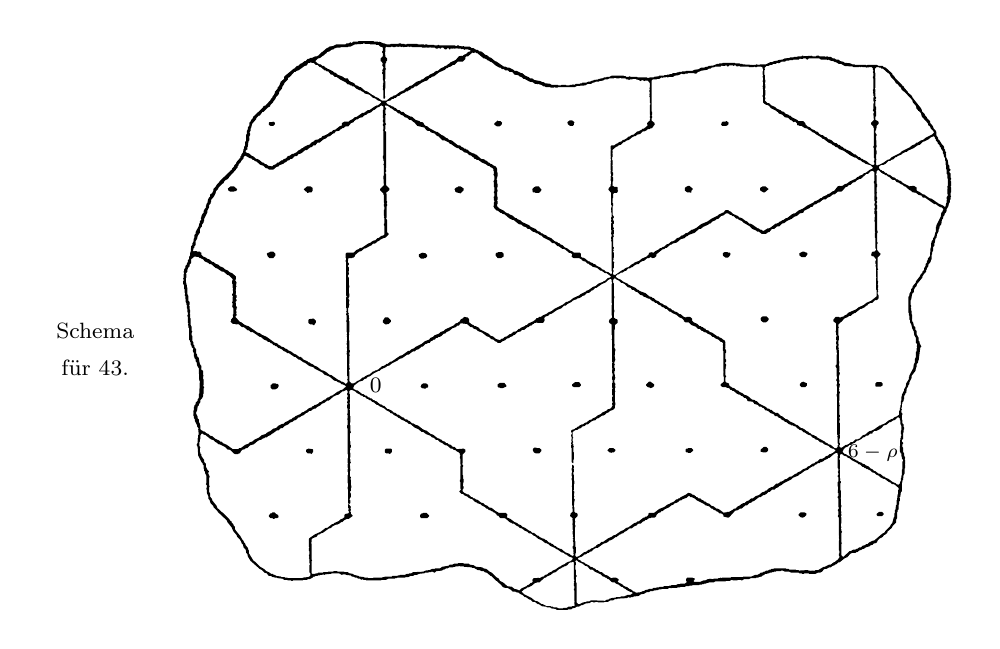
\begin{tikzpicture}[x=.195pt,y=-.195pt]
\path[use as bounding box] (0,0) rectangle (1750,1100);
\path[fill=black,even odd rule] (414,171) -- (413,174) -- (411,176) -- (411,181) -- (408,185) -- (408,188) -- (406,192) -- (406,197) -- (405,198) -- (405,209) -- (403,212) -- (403,218) -- (401,221) -- (401,224) -- (400,225) -- (399,231) -- (396,235) -- (396,237) -- (394,239) -- (394,241) -- (387,249) -- (386,252) -- (383,255) -- (382,258) -- (379,261) -- (379,262) -- (376,265) -- (375,265) -- (374,267) -- (355,285) -- (355,286) -- (351,290) -- (348,295) -- (344,299) -- (344,302) -- (342,306) -- (340,308) -- (339,308) -- (338,310) -- (338,313) -- (336,315) -- (334,319) -- (333,325) -- (331,327) -- (331,329) -- (330,330) -- (330,334) -- (328,336) -- (326,340) -- (326,343) -- (324,345) -- (322,349) -- (322,351) -- (321,352) -- (321,354) -- (322,355) -- (319,359) -- (319,362) -- (318,363) -- (317,368) -- (311,379) -- (311,382) -- (309,384) -- (309,389) -- (308,390) -- (307,397) -- (305,400) -- (305,403) -- (303,405) -- (302,416) -- (301,417) -- (301,422) -- (299,425) -- (299,429) -- (297,431) -- (297,434) -- (295,437) -- (295,439) -- (292,442) -- (292,445) -- (290,448) -- (290,451) -- (289,452) -- (290,456) -- (289,457) -- (289,464) -- (288,465) -- (289,467) -- (289,469) -- (288,470) -- (288,474) -- (290,478) -- (290,484) -- (291,485) -- (291,491) -- (292,492) -- (291,496) -- (292,497) -- (293,509) -- (294,510) -- (294,513) -- (295,514) -- (295,520) -- (296,521) -- (296,527) -- (297,528) -- (297,532) -- (296,533) -- (296,535) -- (297,536) -- (297,547) -- (298,548) -- (297,551) -- (298,552) -- (298,556) -- (299,557) -- (299,578) -- (301,580) -- (301,582) -- (302,583) -- (302,587) -- (304,590) -- (304,592) -- (307,595) -- (306,599) -- (308,603) -- (308,609) -- (309,610) -- (309,612) -- (311,614) -- (311,618) -- (313,620) -- (314,626) -- (317,631) -- (318,654) -- (319,655) -- (318,678) -- (317,679) -- (317,686) -- (315,689) -- (315,691) -- (311,695) -- (311,698) -- (309,700) -- (309,702) -- (308,703) -- (308,709) -- (307,710) -- (307,713) -- (308,714) -- (307,715) -- (307,719) -- (308,720) -- (308,723) -- (310,726) -- (310,729) -- (314,737) -- (314,739) -- (317,743) -- (316,744) -- (317,754) -- (316,755) -- (316,760) -- (315,761) -- (315,763) -- (316,764) -- (315,765) -- (315,769) -- (313,773) -- (315,777) -- (316,793) -- (322,805) -- (324,807) -- (324,809) -- (326,811) -- (326,817) -- (327,818) -- (327,821) -- (329,823) -- (329,826) -- (331,830) -- (331,844) -- (330,846) -- (332,848) -- (332,852) -- (331,853) -- (331,855) -- (332,856) -- (332,862) -- (335,869) -- (335,873) -- (337,875) -- (339,881) -- (344,886) -- (344,888) -- (352,896) -- (352,897) -- (369,913) -- (370,916) -- (378,926) -- (381,933) -- (387,940) -- (388,943) -- (393,948) -- (396,953) -- (396,955) -- (399,958) -- (400,963) -- (404,967) -- (405,973) -- (407,975) -- (408,980) -- (413,988) -- (430,1003) -- (434,1005) -- (439,1010) -- (443,1011) -- (446,1015) -- (448,1016) -- (451,1016) -- (454,1018) -- (457,1018) -- (458,1019) -- (462,1019) -- (463,1020) -- (472,1021) -- (475,1023) -- (481,1023) -- (482,1024) -- (488,1024) -- (489,1025) -- (491,1025) -- (492,1024) -- (510,1024) -- (511,1023) -- (518,1023) -- (519,1022) -- (522,1022) -- (528,1019) -- (530,1017) -- (532,1017) -- (533,1016) -- (537,1016) -- (538,1015) -- (541,1015) -- (542,1014) -- (546,1014) -- (547,1013) -- (550,1014) -- (551,1013) -- (562,1012) -- (563,1011) -- (577,1011) -- (582,1014) -- (584,1013) -- (589,1013) -- (590,1014) -- (599,1015) -- (601,1017) -- (603,1017) -- (607,1019) -- (610,1019) -- (612,1021) -- (616,1021) -- (618,1023) -- (621,1022) -- (622,1023) -- (626,1023) -- (627,1024) -- (655,1024) -- (656,1023) -- (664,1023) -- (668,1021) -- (680,1021) -- (681,1020) -- (684,1020) -- (685,1019) -- (699,1019) -- (700,1018) -- (705,1018) -- (709,1016) -- (714,1016) -- (717,1014) -- (721,1014) -- (725,1012) -- (735,1011) -- (736,1010) -- (742,1010) -- (743,1009) -- (747,1009) -- (748,1008) -- (750,1008) -- (754,1010) -- (757,1007) -- (768,1006) -- (770,1004) -- (772,1004) -- (775,1002) -- (778,1002) -- (781,1000) -- (788,1000) -- (789,999) -- (792,999) -- (793,998) -- (798,998) -- (800,997) -- (801,998) -- (808,998) -- (809,999) -- (823,1000) -- (824,1001) -- (827,1001) -- (834,1005) -- (837,1005) -- (841,1007) -- (845,1007) -- (847,1009) -- (851,1010) -- (858,1016) -- (859,1016) -- (868,1025) -- (869,1025) -- (874,1030) -- (875,1030) -- (881,1037) -- (883,1037) -- (884,1038) -- (889,1038) -- (896,1042) -- (899,1045) -- (904,1045) -- (905,1046) -- (910,1047) -- (912,1049) -- (918,1052) -- (921,1055) -- (923,1055) -- (930,1060) -- (932,1060) -- (936,1064) -- (940,1064) -- (945,1068) -- (947,1068) -- (953,1072) -- (961,1073) -- (962,1074) -- (968,1074) -- (970,1076) -- (978,1077) -- (981,1079) -- (1000,1079) -- (1001,1078) -- (1007,1078) -- (1009,1076) -- (1014,1075) -- (1017,1073) -- (1021,1073) -- (1026,1070) -- (1028,1070) -- (1034,1067) -- (1042,1066) -- (1044,1064) -- (1047,1064) -- (1048,1065) -- (1051,1065) -- (1052,1064) -- (1056,1064) -- (1057,1065) -- (1068,1065) -- (1069,1064) -- (1075,1064) -- (1080,1061) -- (1085,1061) -- (1088,1059) -- (1092,1059) -- (1093,1058) -- (1110,1057) -- (1114,1055) -- (1115,1056) -- (1117,1056) -- (1118,1055) -- (1122,1055) -- (1123,1054) -- (1132,1053) -- (1136,1050) -- (1142,1049) -- (1147,1046) -- (1151,1046) -- (1154,1044) -- (1159,1044) -- (1160,1043) -- (1168,1042) -- (1169,1041) -- (1174,1041) -- (1175,1040) -- (1186,1040) -- (1189,1038) -- (1191,1038) -- (1192,1039) -- (1194,1038) -- (1203,1038) -- (1204,1037) -- (1209,1037) -- (1210,1036) -- (1218,1036) -- (1219,1035) -- (1225,1035) -- (1226,1034) -- (1231,1034) -- (1232,1033) -- (1244,1033) -- (1245,1032) -- (1249,1032) -- (1250,1031) -- (1253,1031) -- (1254,1030) -- (1257,1030) -- (1258,1029) -- (1261,1029) -- (1262,1028) -- (1271,1028) -- (1274,1026) -- (1293,1026) -- (1294,1025) -- (1301,1025) -- (1305,1023) -- (1307,1024) -- (1315,1024) -- (1316,1023) -- (1321,1023) -- (1322,1024) -- (1324,1024) -- (1327,1022) -- (1336,1022) -- (1340,1020) -- (1349,1020) -- (1350,1019) -- (1354,1019) -- (1355,1018) -- (1360,1017) -- (1362,1015) -- (1365,1014) -- (1366,1012) -- (1370,1012) -- (1371,1011) -- (1374,1011) -- (1375,1010) -- (1378,1010) -- (1379,1009) -- (1382,1009) -- (1383,1008) -- (1386,1008) -- (1387,1007) -- (1395,1007) -- (1396,1006) -- (1399,1006) -- (1403,1008) -- (1411,1008) -- (1415,1010) -- (1429,1010) -- (1430,1011) -- (1434,1011) -- (1435,1012) -- (1438,1012) -- (1439,1011) -- (1447,1011) -- (1448,1012) -- (1460,1012) -- (1464,1010) -- (1468,1010) -- (1472,1008) -- (1475,1004) -- (1477,1003) -- (1480,1003) -- (1485,1000) -- (1488,1000) -- (1492,997) -- (1494,997) -- (1496,995) -- (1499,994) -- (1502,991) -- (1504,991) -- (1514,983) -- (1519,981) -- (1524,975) -- (1528,973) -- (1534,973) -- (1535,972) -- (1537,972) -- (1542,968) -- (1544,968) -- (1547,966) -- (1549,966) -- (1553,963) -- (1560,961) -- (1562,959) -- (1566,958) -- (1567,956) -- (1572,955) -- (1574,953) -- (1575,950) -- (1579,946) -- (1581,946) -- (1583,944) -- (1584,944) -- (1587,940) -- (1588,940) -- (1593,936) -- (1593,934) -- (1601,927) -- (1603,923) -- (1609,917) -- (1609,912) -- (1611,909) -- (1611,898) -- (1612,897) -- (1612,894) -- (1614,892) -- (1614,884) -- (1615,883) -- (1615,878) -- (1616,877) -- (1616,872) -- (1615,871) -- (1617,869) -- (1618,861) -- (1620,859) -- (1620,843) -- (1621,842) -- (1621,839) -- (1622,838) -- (1623,829) -- (1625,826) -- (1625,817) -- (1626,816) -- (1626,810) -- (1625,809) -- (1626,808) -- (1626,801) -- (1625,800) -- (1626,797) -- (1624,793) -- (1624,789) -- (1622,786) -- (1622,778) -- (1621,777) -- (1621,774) -- (1620,773) -- (1622,771) -- (1622,769) -- (1620,767) -- (1620,764) -- (1622,762) -- (1622,751) -- (1623,750) -- (1623,745) -- (1624,744) -- (1624,741) -- (1623,740) -- (1623,735) -- (1621,733) -- (1621,727) -- (1620,726) -- (1620,718) -- (1621,717) -- (1621,715) -- (1619,713) -- (1619,709) -- (1620,708) -- (1619,706) -- (1619,704) -- (1620,703) -- (1620,697) -- (1621,696) -- (1621,694) -- (1623,692) -- (1623,689) -- (1624,688) -- (1624,682) -- (1626,680) -- (1626,678) -- (1628,676) -- (1629,668) -- (1631,666) -- (1632,662) -- (1634,660) -- (1634,657) -- (1638,649) -- (1638,645) -- (1645,636) -- (1646,630) -- (1647,629) -- (1647,624) -- (1650,620) -- (1650,617) -- (1651,616) -- (1654,593) -- (1656,591) -- (1653,585) -- (1653,582) -- (1651,580) -- (1651,575) -- (1647,568) -- (1647,562) -- (1645,560) -- (1645,556) -- (1644,554) -- (1642,553) -- (1641,547) -- (1639,544) -- (1639,541) -- (1638,540) -- (1639,539) -- (1639,532) -- (1638,531) -- (1638,525) -- (1637,524) -- (1637,520) -- (1636,519) -- (1637,517) -- (1637,515) -- (1636,514) -- (1636,505) -- (1637,504) -- (1639,493) -- (1642,490) -- (1642,486) -- (1644,482) -- (1647,479) -- (1648,475) -- (1658,463) -- (1658,461) -- (1661,456) -- (1665,452) -- (1665,449) -- (1666,448) -- (1666,446) -- (1669,442) -- (1669,439) -- (1673,434) -- (1674,430) -- (1675,429) -- (1675,421) -- (1676,420) -- (1676,416) -- (1678,412) -- (1678,406) -- (1680,404) -- (1680,399) -- (1681,398) -- (1682,391) -- (1684,389) -- (1685,383) -- (1688,377) -- (1688,374) -- (1689,373) -- (1690,368) -- (1693,364) -- (1694,356) -- (1696,354) -- (1697,349) -- (1699,347) -- (1699,345) -- (1701,343) -- (1703,339) -- (1703,336) -- (1706,331) -- (1707,326) -- (1709,323) -- (1709,319) -- (1710,318) -- (1710,314) -- (1711,313) -- (1710,311) -- (1710,306) -- (1711,305) -- (1711,296) -- (1710,295) -- (1711,293) -- (1711,285) -- (1710,284) -- (1710,282) -- (1711,281) -- (1711,279) -- (1710,278) -- (1710,270) -- (1708,268) -- (1708,266) -- (1710,264) -- (1710,263) -- (1708,261) -- (1708,256) -- (1706,254) -- (1705,246) -- (1702,240) -- (1702,235) -- (1701,234) -- (1702,231) -- (1700,229) -- (1700,226) -- (1698,224) -- (1698,221) -- (1697,219) -- (1694,216) -- (1689,208) -- (1687,207) -- (1687,204) -- (1684,200) -- (1684,194) -- (1682,190) -- (1679,187) -- (1677,182) -- (1672,176) -- (1672,173) -- (1666,167) -- (1666,166) -- (1663,163) -- (1662,160) -- (1657,155) -- (1657,153) -- (1655,149) -- (1640,130) -- (1638,126) -- (1631,120) -- (1631,119) -- (1624,111) -- (1624,110) -- (1622,108) -- (1621,108) -- (1620,106) -- (1608,94) -- (1605,89) -- (1603,88) -- (1602,85) -- (1590,74) -- (1586,73) -- (1584,71) -- (1577,71) -- (1573,69) -- (1556,69) -- (1555,70) -- (1553,69) -- (1533,69) -- (1532,68) -- (1528,68) -- (1524,66) -- (1514,65) -- (1511,63) -- (1506,62) -- (1502,59) -- (1498,59) -- (1495,57) -- (1492,57) -- (1488,54) -- (1483,54) -- (1482,53) -- (1478,54) -- (1477,53) -- (1467,53) -- (1466,52) -- (1462,52) -- (1461,53) -- (1454,53) -- (1453,52) -- (1438,53) -- (1437,52) -- (1435,52) -- (1434,53) -- (1427,53) -- (1426,54) -- (1420,54) -- (1419,55) -- (1413,55) -- (1412,56) -- (1403,57) -- (1399,59) -- (1391,60) -- (1390,61) -- (1383,62) -- (1379,64) -- (1376,64) -- (1368,68) -- (1357,68) -- (1356,69) -- (1350,68) -- (1349,69) -- (1345,69) -- (1344,70) -- (1343,69) -- (1325,68) -- (1324,67) -- (1320,67) -- (1319,66) -- (1311,66) -- (1310,65) -- (1288,65) -- (1287,66) -- (1282,66) -- (1281,67) -- (1278,67) -- (1271,70) -- (1262,71) -- (1261,72) -- (1255,73) -- (1254,74) -- (1248,74) -- (1243,77) -- (1236,78) -- (1232,80) -- (1220,80) -- (1219,81) -- (1213,81) -- (1212,82) -- (1207,82) -- (1206,83) -- (1203,83) -- (1202,84) -- (1196,84) -- (1193,86) -- (1190,86) -- (1189,87) -- (1185,87) -- (1184,88) -- (1180,88) -- (1179,89) -- (1170,89) -- (1169,90) -- (1161,91) -- (1160,92) -- (1153,92) -- (1152,93) -- (1148,93) -- (1147,92) -- (1130,92) -- (1129,91) -- (1117,91) -- (1116,90) -- (1114,91) -- (1109,91) -- (1108,90) -- (1105,90) -- (1104,89) -- (1082,89) -- (1078,91) -- (1073,91) -- (1072,92) -- (1069,92) -- (1065,94) -- (1062,94) -- (1061,95) -- (1058,95) -- (1057,96) -- (1049,97) -- (1048,98) -- (1046,98) -- (1042,100) -- (1039,100) -- (1035,102) -- (1028,102) -- (1027,103) -- (1024,103) -- (1023,104) -- (1016,104) -- (1013,106) -- (1010,105) -- (1009,106) -- (1005,106) -- (1004,107) -- (998,107) -- (997,106) -- (989,106) -- (988,107) -- (983,107) -- (982,106) -- (971,106) -- (968,104) -- (959,103) -- (956,101) -- (954,101) -- (950,99) -- (939,97) -- (935,94) -- (931,94) -- (929,92) -- (922,89) -- (916,84) -- (914,84) -- (906,80) -- (902,80) -- (900,78) -- (892,74) -- (889,74) -- (885,72) -- (882,72) -- (869,63) -- (866,62) -- (859,56) -- (856,55) -- (851,51) -- (849,51) -- (842,45) -- (840,44) -- (837,44) -- (834,41) -- (831,41) -- (826,38) -- (823,38) -- (819,35) -- (809,35) -- (808,34) -- (804,35) -- (803,34) -- (800,34) -- (799,33) -- (796,33) -- (795,34) -- (793,34) -- (792,33) -- (763,33) -- (762,32) -- (760,32) -- (759,33) -- (754,33) -- (753,32) -- (741,32) -- (740,31) -- (737,31) -- (736,32) -- (734,31) -- (728,31) -- (727,32) -- (726,31) -- (723,31) -- (722,30) -- (703,30) -- (702,31) -- (699,31) -- (698,30) -- (692,30) -- (691,29) -- (688,29) -- (687,30) -- (673,30) -- (672,31) -- (665,31) -- (664,30) -- (662,30) -- (661,29) -- (659,29) -- (652,26) -- (650,27) -- (649,26) -- (642,26) -- (641,25) -- (613,25) -- (612,26) -- (603,26) -- (601,28) -- (599,28) -- (598,27) -- (595,29) -- (591,29) -- (589,31) -- (572,31) -- (566,34) -- (559,35) -- (557,37) -- (554,38) -- (546,45) -- (545,45) -- (538,52) -- (536,53) -- (533,53) -- (527,56) -- (524,56) -- (521,58) -- (519,58) -- (515,62) -- (513,62) -- (508,66) -- (505,67) -- (501,71) -- (499,71) -- (494,76) -- (493,76) -- (476,90) -- (475,92) -- (475,95) -- (469,100) -- (466,108) -- (463,111) -- (463,113) -- (458,119) -- (458,121) -- (456,125) -- (454,127) -- (453,130) -- (450,133) -- (450,134) -- (441,144) -- (438,145) -- (436,147) -- (436,148) -- (418,165) -- (417,168) -- cycle (1012,991) -- (1012,1022) -- (1013,1023) -- (1013,1025) -- (1012,1026) -- (1013,1028) -- (1012,1030) -- (1012,1034) -- (1013,1035) -- (1013,1039) -- (1012,1040) -- (1012,1042) -- (1013,1043) -- (1013,1062) -- (1014,1063) -- (1013,1064) -- (1013,1068) -- (1014,1070) -- (1012,1072) -- (1009,1072) -- (1008,1073) -- (1002,1073) -- (999,1075) -- (993,1075) -- (992,1076) -- (984,1076) -- (980,1074) -- (974,1074) -- (973,1073) -- (970,1073) -- (969,1072) -- (962,1072) -- (954,1068) -- (952,1068) -- (945,1063) -- (940,1062) -- (934,1057) -- (920,1050) -- (915,1045) -- (921,1040) -- (924,1039) -- (926,1037) -- (928,1037) -- (934,1034) -- (940,1029) -- (942,1029) -- (943,1028) -- (948,1028) -- (958,1019) -- (960,1019) -- (962,1017) -- (969,1014) -- (974,1010) -- (978,1009) -- (985,1003) -- (988,1002) -- (990,1000) -- (992,1000) -- (994,998) -- (996,998) -- (1000,996) -- (1003,992) -- (1005,991) -- (1008,991) -- (1009,990) -- (1011,990) -- cycle (1015,988) -- (1016,987) -- (1018,987) -- (1021,990) -- (1028,993) -- (1033,997) -- (1037,998) -- (1042,1004) -- (1046,1004) -- (1048,1005) -- (1051,1008) -- (1062,1013) -- (1066,1017) -- (1068,1017) -- (1070,1019) -- (1072,1019) -- (1075,1022) -- (1077,1022) -- (1082,1027) -- (1084,1028) -- (1088,1028) -- (1090,1030) -- (1095,1032) -- (1100,1036) -- (1102,1036) -- (1105,1039) -- (1108,1040) -- (1110,1042) -- (1118,1046) -- (1120,1046) -- (1121,1048) -- (1117,1051) -- (1112,1051) -- (1105,1054) -- (1099,1054) -- (1098,1055) -- (1091,1055) -- (1090,1056) -- (1081,1057) -- (1080,1058) -- (1078,1058) -- (1076,1060) -- (1073,1060) -- (1070,1062) -- (1044,1061) -- (1041,1063) -- (1036,1063) -- (1035,1064) -- (1029,1065) -- (1023,1068) -- (1020,1068) -- (1017,1065) -- (1017,1029) -- (1016,1028) -- (1016,1018) -- (1017,1017) -- (1017,1015) -- (1016,1014) -- (1016,1005) -- (1015,1004) -- (1015,996) -- (1016,995) -- (1016,991) -- (1015,990) -- cycle (1507,790) -- (1509,790) -- (1511,792) -- (1515,794) -- (1517,794) -- (1520,797) -- (1523,798) -- (1528,802) -- (1538,807) -- (1540,809) -- (1542,809) -- (1547,814) -- (1549,814) -- (1551,816) -- (1553,816) -- (1555,818) -- (1557,818) -- (1559,820) -- (1561,820) -- (1565,824) -- (1569,825) -- (1572,828) -- (1577,830) -- (1580,833) -- (1586,836) -- (1588,836) -- (1596,842) -- (1599,843) -- (1602,846) -- (1605,846) -- (1607,847) -- (1614,853) -- (1614,856) -- (1613,857) -- (1613,864) -- (1612,865) -- (1611,875) -- (1610,876) -- (1610,884) -- (1609,885) -- (1608,893) -- (1607,894) -- (1607,899) -- (1606,900) -- (1606,906) -- (1605,907) -- (1602,918) -- (1600,920) -- (1598,924) -- (1589,933) -- (1589,934) -- (1587,936) -- (1583,938) -- (1569,950) -- (1565,951) -- (1559,954) -- (1556,957) -- (1554,957) -- (1551,959) -- (1547,960) -- (1544,963) -- (1541,963) -- (1537,966) -- (1535,966) -- (1534,967) -- (1530,967) -- (1525,970) -- (1523,970) -- (1511,981) -- (1508,978) -- (1508,956) -- (1509,955) -- (1508,954) -- (1508,936) -- (1509,934) -- (1508,933) -- (1508,930) -- (1507,929) -- (1507,927) -- (1508,926) -- (1507,924) -- (1507,919) -- (1508,918) -- (1508,908) -- (1507,907) -- (1507,905) -- (1508,904) -- (1508,902) -- (1507,901) -- (1508,897) -- (1507,896) -- (1507,889) -- (1508,888) -- (1508,885) -- (1507,884) -- (1507,873) -- (1506,872) -- (1507,870) -- (1507,858) -- (1506,857) -- (1506,844) -- (1507,843) -- (1507,841) -- (1505,839) -- (1506,836) -- (1505,835) -- (1505,820) -- (1504,819) -- (1505,818) -- (1505,801) -- (1504,800) -- (1504,798) -- (1505,797) -- (1505,792) -- cycle (1573,901) -- (1573,903) -- (1575,905) -- (1583,905) -- (1586,902) -- (1586,900) -- (1583,897) -- (1578,897) -- cycle (1501,789) -- (1501,791) -- (1502,792) -- (1501,794) -- (1501,816) -- (1502,817) -- (1502,822) -- (1501,823) -- (1502,825) -- (1502,829) -- (1501,830) -- (1501,832) -- (1502,833) -- (1502,841) -- (1501,842) -- (1501,850) -- (1502,851) -- (1501,861) -- (1502,862) -- (1502,868) -- (1501,869) -- (1501,871) -- (1502,872) -- (1502,888) -- (1503,889) -- (1503,891) -- (1501,894) -- (1502,896) -- (1502,903) -- (1501,905) -- (1503,908) -- (1503,941) -- (1504,942) -- (1503,944) -- (1504,946) -- (1503,947) -- (1504,949) -- (1503,951) -- (1503,968) -- (1504,969) -- (1504,974) -- (1503,975) -- (1503,978) -- (1504,979) -- (1504,982) -- (1500,987) -- (1499,987) -- (1496,990) -- (1493,991) -- (1488,995) -- (1485,995) -- (1477,999) -- (1475,999) -- (1465,1005) -- (1460,1005) -- (1457,1007) -- (1456,1006) -- (1453,1006) -- (1451,1007) -- (1450,1006) -- (1447,1006) -- (1446,1005) -- (1429,1006) -- (1428,1005) -- (1424,1005) -- (1423,1004) -- (1411,1004) -- (1410,1003) -- (1406,1003) -- (1405,1002) -- (1383,1002) -- (1382,1003) -- (1378,1003) -- (1377,1004) -- (1375,1004) -- (1372,1006) -- (1368,1006) -- (1366,1008) -- (1364,1008) -- (1361,1010) -- (1358,1010) -- (1356,1012) -- (1352,1014) -- (1348,1014) -- (1341,1017) -- (1326,1017) -- (1325,1018) -- (1304,1018) -- (1303,1019) -- (1287,1019) -- (1286,1020) -- (1284,1019) -- (1283,1020) -- (1280,1020) -- (1279,1021) -- (1271,1021) -- (1270,1022) -- (1264,1021) -- (1263,1022) -- (1260,1022) -- (1256,1024) -- (1253,1024) -- (1246,1027) -- (1235,1027) -- (1234,1026) -- (1234,1025) -- (1236,1023) -- (1236,1021) -- (1235,1020) -- (1233,1020) -- (1232,1019) -- (1222,1019) -- (1220,1022) -- (1220,1025) -- (1222,1027) -- (1218,1030) -- (1210,1030) -- (1209,1031) -- (1205,1031) -- (1201,1033) -- (1193,1033) -- (1192,1034) -- (1189,1034) -- (1188,1035) -- (1179,1035) -- (1178,1036) -- (1171,1036) -- (1170,1037) -- (1166,1037) -- (1165,1038) -- (1160,1038) -- (1157,1040) -- (1151,1040) -- (1150,1041) -- (1145,1042) -- (1142,1044) -- (1140,1044) -- (1136,1046) -- (1127,1047) -- (1125,1045) -- (1123,1045) -- (1118,1041) -- (1115,1040) -- (1110,1036) -- (1108,1036) -- (1104,1034) -- (1101,1031) -- (1095,1028) -- (1093,1026) -- (1095,1024) -- (1095,1022) -- (1090,1019) -- (1084,1019) -- (1083,1020) -- (1081,1020) -- (1074,1015) -- (1070,1014) -- (1064,1009) -- (1062,1009) -- (1058,1007) -- (1056,1005) -- (1054,1005) -- (1051,1002) -- (1049,1002) -- (1047,1000) -- (1043,999) -- (1041,997) -- (1033,993) -- (1031,991) -- (1027,990) -- (1024,987) -- (1021,986) -- (1019,984) -- (1021,982) -- (1027,980) -- (1032,976) -- (1034,976) -- (1038,973) -- (1040,973) -- (1042,971) -- (1046,970) -- (1046,969) -- (1049,966) -- (1053,964) -- (1056,964) -- (1067,956) -- (1071,955) -- (1075,953) -- (1078,950) -- (1080,950) -- (1084,948) -- (1089,944) -- (1091,944) -- (1094,941) -- (1095,941) -- (1097,939) -- (1099,939) -- (1101,937) -- (1103,937) -- (1106,934) -- (1109,933) -- (1115,928) -- (1119,928) -- (1124,924) -- (1129,922) -- (1130,920) -- (1132,919) -- (1136,919) -- (1140,915) -- (1142,915) -- (1145,912) -- (1147,912) -- (1151,909) -- (1154,909) -- (1155,908) -- (1161,908) -- (1163,907) -- (1165,905) -- (1165,903) -- (1169,899) -- (1173,898) -- (1174,896) -- (1176,896) -- (1181,892) -- (1188,889) -- (1193,885) -- (1196,884) -- (1199,881) -- (1201,881) -- (1205,879) -- (1208,876) -- (1211,876) -- (1213,874) -- (1221,871) -- (1224,868) -- (1227,868) -- (1228,870) -- (1231,870) -- (1237,873) -- (1240,876) -- (1254,883) -- (1256,885) -- (1263,887) -- (1267,891) -- (1269,891) -- (1272,894) -- (1274,894) -- (1276,896) -- (1279,897) -- (1282,900) -- (1285,900) -- (1287,901) -- (1289,903) -- (1289,905) -- (1290,906) -- (1298,908) -- (1300,907) -- (1311,895) -- (1316,894) -- (1320,891) -- (1323,891) -- (1330,885) -- (1333,885) -- (1337,881) -- (1341,880) -- (1343,878) -- (1346,877) -- (1355,870) -- (1358,870) -- (1363,866) -- (1365,866) -- (1369,864) -- (1373,860) -- (1375,860) -- (1379,856) -- (1384,856) -- (1387,853) -- (1390,852) -- (1393,849) -- (1396,848) -- (1401,844) -- (1415,837) -- (1418,834) -- (1428,830) -- (1431,827) -- (1432,827) -- (1440,821) -- (1446,819) -- (1449,816) -- (1454,813) -- (1456,813) -- (1459,810) -- (1462,809) -- (1464,807) -- (1467,807) -- (1469,805) -- (1471,805) -- (1475,803) -- (1477,801) -- (1482,799) -- (1484,797) -- (1486,797) -- (1494,790) -- (1498,788) -- (1500,788) -- cycle (1428,903) -- (1432,907) -- (1436,908) -- (1440,906) -- (1443,903) -- (1443,900) -- (1439,898) -- (1433,898) -- (1431,899) -- cycle (1612,722) -- (1614,722) -- (1616,724) -- (1616,727) -- (1617,728) -- (1617,734) -- (1619,738) -- (1619,746) -- (1618,747) -- (1618,753) -- (1619,754) -- (1619,756) -- (1618,757) -- (1618,760) -- (1617,761) -- (1616,785) -- (1617,786) -- (1617,788) -- (1619,789) -- (1619,794) -- (1620,795) -- (1620,798) -- (1622,801) -- (1622,803) -- (1621,804) -- (1621,818) -- (1620,819) -- (1620,829) -- (1619,830) -- (1619,834) -- (1618,835) -- (1618,840) -- (1617,841) -- (1616,845) -- (1614,847) -- (1610,846) -- (1608,844) -- (1603,842) -- (1595,836) -- (1590,834) -- (1588,832) -- (1586,832) -- (1580,827) -- (1576,826) -- (1571,822) -- (1568,821) -- (1565,818) -- (1562,817) -- (1558,813) -- (1553,811) -- (1551,809) -- (1547,808) -- (1545,806) -- (1541,805) -- (1537,802) -- (1535,802) -- (1533,800) -- (1530,799) -- (1523,794) -- (1518,792) -- (1516,790) -- (1514,790) -- (1510,786) -- (1512,781) -- (1515,778) -- (1520,776) -- (1523,773) -- (1526,773) -- (1528,771) -- (1533,769) -- (1537,765) -- (1539,765) -- (1545,762) -- (1548,759) -- (1550,759) -- (1554,756) -- (1557,756) -- (1561,752) -- (1565,752) -- (1565,751) -- (1569,747) -- (1573,747) -- (1579,744) -- (1581,742) -- (1582,742) -- (1586,737) -- (1591,736) -- (1597,731) -- (1599,731) -- (1603,728) -- (1607,727) -- cycle (596,673) -- (599,671) -- (603,672) -- (607,674) -- (610,677) -- (616,680) -- (618,682) -- (620,682) -- (622,684) -- (625,684) -- (629,688) -- (631,688) -- (633,690) -- (635,690) -- (638,693) -- (641,694) -- (647,699) -- (649,699) -- (651,701) -- (660,705) -- (665,709) -- (671,712) -- (672,714) -- (676,715) -- (679,718) -- (685,721) -- (687,723) -- (690,724) -- (692,726) -- (699,729) -- (701,731) -- (703,731) -- (706,734) -- (710,735) -- (717,741) -- (724,744) -- (730,749) -- (733,749) -- (738,753) -- (746,756) -- (749,759) -- (753,760) -- (757,764) -- (760,764) -- (764,768) -- (769,770) -- (771,772) -- (775,774) -- (777,774) -- (784,780) -- (787,780) -- (789,782) -- (793,783) -- (795,785) -- (799,787) -- (801,789) -- (801,792) -- (802,793) -- (801,795) -- (801,798) -- (802,799) -- (802,809) -- (803,810) -- (802,812) -- (802,837) -- (801,838) -- (801,841) -- (802,842) -- (802,854) -- (803,856) -- (800,859) -- (800,860) -- (804,864) -- (807,864) -- (810,867) -- (815,869) -- (817,871) -- (821,873) -- (823,873) -- (829,879) -- (831,879) -- (833,881) -- (839,883) -- (841,885) -- (847,888) -- (850,891) -- (852,891) -- (855,894) -- (857,894) -- (859,896) -- (861,896) -- (863,898) -- (866,899) -- (869,902) -- (869,903) -- (870,904) -- (872,904) -- (875,908) -- (877,909) -- (884,909) -- (886,910) -- (894,917) -- (896,917) -- (898,919) -- (901,919) -- (906,923) -- (909,924) -- (912,927) -- (916,928) -- (921,932) -- (926,934) -- (929,937) -- (932,937) -- (934,938) -- (937,941) -- (940,942) -- (946,947) -- (953,950) -- (959,955) -- (961,955) -- (965,957) -- (968,960) -- (977,964) -- (979,966) -- (982,967) -- (989,972) -- (993,973) -- (996,976) -- (998,976) -- (1003,980) -- (1009,982) -- (1010,983) -- (1009,986) -- (1005,989) -- (1001,990) -- (997,992) -- (995,994) -- (990,996) -- (988,998) -- (985,999) -- (978,1004) -- (973,1006) -- (971,1008) -- (966,1010) -- (963,1013) -- (959,1014) -- (956,1017) -- (954,1017) -- (949,1020) -- (947,1020) -- (946,1019) -- (944,1020) -- (937,1020) -- (937,1021) -- (935,1023) -- (936,1027) -- (934,1029) -- (932,1029) -- (929,1032) -- (926,1033) -- (924,1035) -- (915,1039) -- (911,1043) -- (907,1041) -- (902,1040) -- (897,1036) -- (889,1035) -- (881,1028) -- (875,1025) -- (873,1021) -- (868,1018) -- (860,1010) -- (856,1008) -- (850,1003) -- (845,1002) -- (842,1000) -- (831,999) -- (826,996) -- (819,995) -- (817,993) -- (808,993) -- (807,992) -- (798,992) -- (797,993) -- (791,993) -- (787,995) -- (782,995) -- (780,997) -- (768,999) -- (764,1002) -- (755,1002) -- (754,1003) -- (749,1003) -- (745,1005) -- (737,1006) -- (733,1008) -- (714,1009) -- (711,1011) -- (707,1011) -- (706,1012) -- (703,1012) -- (699,1014) -- (690,1014) -- (689,1015) -- (686,1015) -- (685,1016) -- (676,1016) -- (675,1017) -- (662,1017) -- (661,1018) -- (658,1018) -- (657,1019) -- (641,1019) -- (640,1020) -- (631,1020) -- (630,1019) -- (624,1019) -- (623,1018) -- (614,1017) -- (613,1016) -- (605,1014) -- (602,1012) -- (596,1011) -- (593,1009) -- (587,1009) -- (586,1008) -- (574,1008) -- (573,1007) -- (567,1007) -- (566,1008) -- (557,1008) -- (556,1009) -- (548,1009) -- (547,1010) -- (538,1010) -- (537,1011) -- (534,1011) -- (533,1012) -- (527,1012) -- (526,1011) -- (526,989) -- (527,987) -- (526,986) -- (526,956) -- (525,955) -- (526,953) -- (526,948) -- (528,946) -- (536,943) -- (536,942) -- (539,939) -- (541,939) -- (543,937) -- (547,936) -- (558,928) -- (562,927) -- (565,924) -- (571,921) -- (573,921) -- (579,918) -- (581,916) -- (583,916) -- (586,913) -- (592,910) -- (595,910) -- (602,905) -- (602,904) -- (599,901) -- (599,898) -- (598,897) -- (598,895) -- (599,894) -- (598,890) -- (599,888) -- (595,883) -- (598,881) -- (598,876) -- (596,874) -- (599,869) -- (599,864) -- (597,860) -- (599,858) -- (599,853) -- (600,852) -- (600,849) -- (599,848) -- (599,838) -- (598,837) -- (599,833) -- (597,831) -- (597,822) -- (598,821) -- (597,808) -- (599,806) -- (598,804) -- (598,800) -- (597,799) -- (597,797) -- (598,796) -- (598,788) -- (597,787) -- (597,784) -- (598,782) -- (597,780) -- (599,777) -- (599,774) -- (598,773) -- (598,767) -- (597,766) -- (597,752) -- (599,750) -- (599,749) -- (598,748) -- (598,737) -- (597,736) -- (597,732) -- (598,731) -- (598,720) -- (597,719) -- (597,709) -- (596,708) -- (597,706) -- (597,697) -- (596,696) -- (597,694) -- (597,690) -- (596,689) -- (597,688) -- (597,679) -- (596,678) -- cycle (727,903) -- (727,906) -- (729,909) -- (740,909) -- (744,905) -- (744,904) -- (739,899) -- (733,899) -- (732,900) -- (730,900) -- cycle (662,782) -- (662,787) -- (665,789) -- (669,789) -- (671,790) -- (675,786) -- (675,782) -- (673,780) -- (664,780) -- cycle (591,671) -- (593,674) -- (593,677) -- (592,678) -- (592,680) -- (593,681) -- (593,684) -- (592,685) -- (592,688) -- (593,689) -- (593,692) -- (592,693) -- (592,695) -- (593,696) -- (593,698) -- (592,699) -- (592,705) -- (593,706) -- (593,715) -- (592,716) -- (593,718) -- (593,724) -- (592,725) -- (593,727) -- (593,736) -- (592,737) -- (592,742) -- (593,743) -- (593,790) -- (594,791) -- (594,797) -- (593,798) -- (593,807) -- (594,808) -- (593,809) -- (593,815) -- (594,816) -- (593,818) -- (593,823) -- (594,824) -- (594,828) -- (593,829) -- (593,844) -- (594,845) -- (594,850) -- (593,851) -- (593,855) -- (594,856) -- (594,881) -- (595,882) -- (594,884) -- (594,890) -- (595,891) -- (594,895) -- (595,896) -- (595,899) -- (594,900) -- (589,901) -- (587,903) -- (587,907) -- (583,910) -- (580,911) -- (577,914) -- (568,918) -- (566,920) -- (564,920) -- (555,927) -- (552,927) -- (543,934) -- (532,939) -- (522,946) -- (521,948) -- (521,962) -- (522,963) -- (521,965) -- (521,969) -- (522,970) -- (522,976) -- (521,977) -- (522,981) -- (521,983) -- (522,984) -- (522,992) -- (523,993) -- (523,995) -- (522,996) -- (522,1009) -- (524,1011) -- (524,1015) -- (522,1017) -- (520,1018) -- (510,1019) -- (509,1020) -- (482,1020) -- (481,1019) -- (477,1019) -- (476,1018) -- (470,1018) -- (469,1017) -- (461,1016) -- (458,1014) -- (456,1014) -- (454,1012) -- (451,1012) -- (447,1009) -- (442,1007) -- (438,1003) -- (431,999) -- (421,989) -- (420,989) -- (418,987) -- (410,974) -- (410,969) -- (409,968) -- (408,964) -- (404,959) -- (403,956) -- (401,954) -- (400,951) -- (398,949) -- (394,942) -- (385,931) -- (384,929) -- (384,925) -- (382,923) -- (381,920) -- (378,917) -- (378,915) -- (376,914) -- (374,912) -- (374,911) -- (361,898) -- (360,898) -- (354,892) -- (352,891) -- (350,886) -- (342,876) -- (342,874) -- (338,869) -- (338,863) -- (336,860) -- (336,852) -- (337,851) -- (337,849) -- (336,848) -- (336,834) -- (337,833) -- (337,831) -- (335,827) -- (335,824) -- (336,822) -- (333,819) -- (330,813) -- (330,808) -- (328,806) -- (327,804) -- (327,801) -- (322,794) -- (322,791) -- (320,789) -- (320,787) -- (319,786) -- (319,780) -- (320,778) -- (318,775) -- (318,768) -- (319,767) -- (319,763) -- (320,762) -- (320,756) -- (321,754) -- (323,752) -- (324,752) -- (326,754) -- (330,755) -- (333,758) -- (334,758) -- (336,760) -- (336,761) -- (338,761) -- (340,763) -- (344,764) -- (348,768) -- (349,768) -- (354,772) -- (356,772) -- (366,777) -- (371,782) -- (374,782) -- (376,783) -- (382,789) -- (384,790) -- (390,790) -- (391,789) -- (393,789) -- (395,785) -- (398,782) -- (402,781) -- (404,779) -- (407,779) -- (412,774) -- (419,772) -- (426,766) -- (430,764) -- (432,764) -- (436,761) -- (438,761) -- (440,759) -- (443,759) -- (445,757) -- (450,755) -- (453,752) -- (454,752) -- (462,746) -- (465,746) -- (469,742) -- (472,742) -- (476,738) -- (483,735) -- (486,732) -- (491,730) -- (493,728) -- (497,727) -- (502,722) -- (504,722) -- (508,719) -- (510,719) -- (516,714) -- (519,713) -- (522,710) -- (525,710) -- (527,708) -- (531,706) -- (533,706) -- (536,703) -- (542,700) -- (545,697) -- (550,695) -- (555,691) -- (558,691) -- (566,684) -- (572,681) -- (576,680) -- (583,674) -- (585,674) -- cycle (447,904) -- (447,906) -- (450,909) -- (454,909) -- (455,910) -- (457,910) -- (458,909) -- (462,909) -- (465,907) -- (464,903) -- (460,901) -- (457,898) -- (454,898) -- (452,900) -- (450,900) -- cycle (516,782) -- (516,786) -- (519,789) -- (524,789) -- (526,790) -- (529,786) -- (529,782) -- (528,781) -- (520,780) -- cycle (1497,784) -- (1492,788) -- (1488,790) -- (1486,790) -- (1483,793) -- (1479,794) -- (1476,797) -- (1472,799) -- (1469,799) -- (1467,800) -- (1463,804) -- (1461,804) -- (1458,807) -- (1454,808) -- (1449,812) -- (1446,813) -- (1443,816) -- (1437,818) -- (1432,822) -- (1427,824) -- (1425,826) -- (1422,827) -- (1415,832) -- (1412,832) -- (1407,836) -- (1403,837) -- (1401,839) -- (1397,841) -- (1395,841) -- (1392,844) -- (1390,845) -- (1387,845) -- (1381,851) -- (1379,851) -- (1373,854) -- (1369,858) -- (1367,858) -- (1365,860) -- (1361,861) -- (1355,866) -- (1349,868) -- (1344,872) -- (1341,872) -- (1335,877) -- (1333,877) -- (1328,881) -- (1326,881) -- (1322,883) -- (1320,885) -- (1316,887) -- (1312,891) -- (1309,891) -- (1307,893) -- (1300,897) -- (1296,897) -- (1295,898) -- (1292,898) -- (1290,899) -- (1282,893) -- (1278,891) -- (1276,891) -- (1271,887) -- (1267,886) -- (1263,882) -- (1259,881) -- (1256,878) -- (1254,878) -- (1252,876) -- (1249,875) -- (1246,872) -- (1243,872) -- (1241,870) -- (1239,870) -- (1238,868) -- (1237,868) -- (1235,866) -- (1231,865) -- (1229,863) -- (1224,862) -- (1220,865) -- (1210,870) -- (1208,872) -- (1206,872) -- (1204,874) -- (1202,874) -- (1198,878) -- (1194,880) -- (1192,880) -- (1190,882) -- (1185,884) -- (1180,888) -- (1170,892) -- (1161,899) -- (1152,899) -- (1150,901) -- (1150,903) -- (1147,906) -- (1145,906) -- (1143,908) -- (1141,908) -- (1132,915) -- (1130,915) -- (1128,917) -- (1124,918) -- (1113,926) -- (1109,927) -- (1104,931) -- (1099,933) -- (1089,940) -- (1085,941) -- (1083,943) -- (1076,946) -- (1066,953) -- (1063,953) -- (1059,957) -- (1057,957) -- (1055,959) -- (1054,959) -- (1053,961) -- (1050,962) -- (1048,964) -- (1044,965) -- (1042,967) -- (1040,967) -- (1035,971) -- (1031,972) -- (1022,979) -- (1017,981) -- (1015,979) -- (1015,974) -- (1016,973) -- (1016,963) -- (1015,962) -- (1015,952) -- (1014,951) -- (1014,926) -- (1015,925) -- (1015,922) -- (1014,921) -- (1014,917) -- (1015,916) -- (1014,914) -- (1014,910) -- (1019,905) -- (1019,901) -- (1017,899) -- (1015,899) -- (1013,897) -- (1013,889) -- (1012,888) -- (1013,877) -- (1014,875) -- (1012,872) -- (1012,870) -- (1013,869) -- (1012,867) -- (1013,860) -- (1011,858) -- (1012,856) -- (1012,846) -- (1013,845) -- (1013,840) -- (1012,839) -- (1012,829) -- (1011,828) -- (1011,824) -- (1012,823) -- (1012,818) -- (1011,817) -- (1012,816) -- (1012,812) -- (1010,810) -- (1009,810) -- (1009,816) -- (1008,817) -- (1008,820) -- (1009,821) -- (1009,824) -- (1008,825) -- (1008,831) -- (1009,832) -- (1009,834) -- (1008,835) -- (1008,838) -- (1009,839) -- (1009,848) -- (1008,850) -- (1009,851) -- (1009,885) -- (1010,886) -- (1009,890) -- (1010,891) -- (1010,897) -- (1006,900) -- (1006,902) -- (1005,903) -- (1005,905) -- (1010,909) -- (1010,911) -- (1009,912) -- (1010,913) -- (1010,918) -- (1009,920) -- (1010,921) -- (1010,930) -- (1011,931) -- (1010,933) -- (1010,939) -- (1011,940) -- (1010,942) -- (1011,944) -- (1011,946) -- (1010,947) -- (1011,948) -- (1011,950) -- (1010,951) -- (1011,953) -- (1011,960) -- (1010,961) -- (1010,965) -- (1011,966) -- (1011,972) -- (1012,973) -- (1011,974) -- (1012,977) -- (1010,979) -- (1006,977) -- (1004,975) -- (996,972) -- (989,966) -- (987,966) -- (981,963) -- (979,961) -- (976,960) -- (973,957) -- (970,956) -- (968,954) -- (966,954) -- (962,950) -- (959,949) -- (957,947) -- (955,947) -- (949,944) -- (946,941) -- (944,941) -- (938,936) -- (935,936) -- (932,933) -- (929,932) -- (922,927) -- (917,925) -- (914,922) -- (909,920) -- (907,918) -- (902,916) -- (894,910) -- (889,908) -- (888,907) -- (889,902) -- (886,899) -- (873,899) -- (866,895) -- (860,890) -- (855,889) -- (852,886) -- (847,884) -- (844,881) -- (840,880) -- (834,875) -- (830,874) -- (828,872) -- (826,872) -- (824,870) -- (822,870) -- (817,865) -- (815,865) -- (809,862) -- (806,859) -- (806,856) -- (808,853) -- (808,851) -- (806,848) -- (807,846) -- (807,843) -- (808,842) -- (808,837) -- (807,836) -- (807,830) -- (806,829) -- (806,814) -- (807,813) -- (807,811) -- (805,809) -- (805,808) -- (806,807) -- (806,791) -- (811,786) -- (811,782) -- (808,780) -- (795,781) -- (791,777) -- (788,777) -- (784,773) -- (780,772) -- (778,770) -- (776,770) -- (773,767) -- (769,766) -- (766,763) -- (764,763) -- (762,761) -- (760,761) -- (751,754) -- (747,753) -- (738,746) -- (736,746) -- (732,744) -- (723,737) -- (719,736) -- (714,733) -- (712,733) -- (708,729) -- (705,728) -- (703,726) -- (700,726) -- (696,722) -- (694,722) -- (687,717) -- (685,717) -- (682,714) -- (678,713) -- (675,710) -- (669,707) -- (667,707) -- (661,701) -- (659,701) -- (655,698) -- (653,698) -- (646,692) -- (644,692) -- (642,690) -- (640,690) -- (637,687) -- (635,687) -- (633,685) -- (631,685) -- (628,682) -- (626,682) -- (622,679) -- (620,679) -- (611,672) -- (609,672) -- (605,670) -- (603,668) -- (605,663) -- (614,656) -- (621,654) -- (624,651) -- (628,650) -- (628,649) -- (630,647) -- (634,646) -- (642,640) -- (650,636) -- (652,636) -- (655,633) -- (664,629) -- (666,627) -- (670,626) -- (675,622) -- (685,617) -- (687,615) -- (691,613) -- (693,613) -- (703,606) -- (706,606) -- (712,601) -- (714,600) -- (717,600) -- (720,597) -- (724,596) -- (730,591) -- (732,591) -- (737,586) -- (739,586) -- (742,584) -- (745,584) -- (747,581) -- (750,580) -- (752,578) -- (755,578) -- (755,577) -- (757,575) -- (759,575) -- (761,573) -- (763,573) -- (767,571) -- (771,567) -- (774,567) -- (774,566) -- (776,564) -- (781,562) -- (787,557) -- (793,555) -- (796,552) -- (799,552) -- (802,548) -- (807,548) -- (808,549) -- (810,548) -- (811,549) -- (814,549) -- (821,555) -- (824,555) -- (827,558) -- (831,559) -- (834,562) -- (842,565) -- (851,572) -- (855,573) -- (859,577) -- (863,578) -- (866,581) -- (869,582) -- (871,584) -- (876,584) -- (880,581) -- (885,579) -- (888,576) -- (892,575) -- (894,573) -- (898,572) -- (900,570) -- (903,569) -- (908,564) -- (913,563) -- (916,560) -- (920,560) -- (926,555) -- (928,555) -- (931,552) -- (933,552) -- (936,549) -- (938,549) -- (939,547) -- (942,547) -- (943,546) -- (945,547) -- (954,547) -- (956,546) -- (958,542) -- (957,538) -- (960,535) -- (964,534) -- (967,531) -- (971,530) -- (981,523) -- (989,520) -- (994,515) -- (997,515) -- (1000,512) -- (1008,508) -- (1010,506) -- (1014,504) -- (1016,504) -- (1018,502) -- (1022,501) -- (1026,499) -- (1028,497) -- (1032,496) -- (1036,492) -- (1041,491) -- (1045,487) -- (1047,487) -- (1052,482) -- (1054,482) -- (1064,475) -- (1071,472) -- (1075,468) -- (1080,465) -- (1082,467) -- (1082,471) -- (1083,472) -- (1083,474) -- (1082,475) -- (1082,510) -- (1083,511) -- (1083,513) -- (1082,514) -- (1082,533) -- (1083,534) -- (1083,537) -- (1078,541) -- (1077,545) -- (1078,547) -- (1082,550) -- (1082,569) -- (1083,570) -- (1083,576) -- (1082,578) -- (1083,579) -- (1083,619) -- (1084,620) -- (1083,622) -- (1083,631) -- (1084,632) -- (1083,634) -- (1083,640) -- (1084,641) -- (1084,646) -- (1083,647) -- (1083,652) -- (1084,653) -- (1084,658) -- (1083,659) -- (1083,667) -- (1084,668) -- (1083,670) -- (1083,680) -- (1084,681) -- (1084,684) -- (1083,685) -- (1083,692) -- (1084,693) -- (1084,695) -- (1083,696) -- (1083,698) -- (1084,700) -- (1081,705) -- (1077,707) -- (1075,707) -- (1072,710) -- (1065,713) -- (1062,716) -- (1057,718) -- (1052,722) -- (1047,724) -- (1045,726) -- (1041,727) -- (1035,732) -- (1033,732) -- (1029,735) -- (1027,735) -- (1023,737) -- (1021,739) -- (1018,740) -- (1017,742) -- (1015,742) -- (1013,744) -- (1009,745) -- (1007,747) -- (1007,749) -- (1009,751) -- (1007,755) -- (1007,757) -- (1008,758) -- (1008,763) -- (1007,764) -- (1008,766) -- (1008,768) -- (1007,769) -- (1007,771) -- (1008,772) -- (1007,774) -- (1007,778) -- (1008,779) -- (1008,805) -- (1010,807) -- (1011,807) -- (1011,801) -- (1012,800) -- (1012,787) -- (1011,786) -- (1011,778) -- (1012,776) -- (1011,775) -- (1011,772) -- (1010,771) -- (1010,769) -- (1011,768) -- (1010,766) -- (1010,761) -- (1011,760) -- (1010,758) -- (1010,749) -- (1014,746) -- (1019,745) -- (1021,743) -- (1025,742) -- (1028,739) -- (1032,738) -- (1035,735) -- (1038,735) -- (1044,730) -- (1048,728) -- (1053,727) -- (1053,726) -- (1055,724) -- (1057,724) -- (1064,719) -- (1066,719) -- (1070,717) -- (1073,714) -- (1076,713) -- (1079,710) -- (1085,708) -- (1088,705) -- (1088,700) -- (1089,699) -- (1089,695) -- (1088,694) -- (1088,675) -- (1089,674) -- (1088,672) -- (1088,668) -- (1089,667) -- (1089,665) -- (1088,663) -- (1089,662) -- (1089,660) -- (1087,657) -- (1087,653) -- (1088,652) -- (1089,648) -- (1088,647) -- (1088,643) -- (1087,642) -- (1087,637) -- (1088,636) -- (1088,631) -- (1087,630) -- (1087,626) -- (1088,624) -- (1087,623) -- (1087,619) -- (1088,618) -- (1089,614) -- (1088,613) -- (1088,610) -- (1087,608) -- (1088,607) -- (1088,600) -- (1089,599) -- (1089,596) -- (1087,593) -- (1087,589) -- (1088,588) -- (1087,586) -- (1087,560) -- (1088,559) -- (1088,551) -- (1093,547) -- (1093,542) -- (1092,540) -- (1090,540) -- (1086,537) -- (1086,528) -- (1087,527) -- (1087,523) -- (1086,522) -- (1086,502) -- (1087,501) -- (1087,498) -- (1086,497) -- (1086,474) -- (1085,473) -- (1085,467) -- (1088,464) -- (1090,466) -- (1096,469) -- (1100,473) -- (1102,473) -- (1106,475) -- (1112,481) -- (1117,482) -- (1120,486) -- (1123,486) -- (1126,489) -- (1130,490) -- (1135,495) -- (1139,496) -- (1142,499) -- (1144,499) -- (1150,502) -- (1152,502) -- (1158,507) -- (1160,507) -- (1163,510) -- (1165,510) -- (1170,514) -- (1172,514) -- (1176,518) -- (1178,518) -- (1182,521) -- (1184,521) -- (1189,526) -- (1191,526) -- (1195,529) -- (1202,532) -- (1208,537) -- (1213,539) -- (1216,542) -- (1216,544) -- (1219,546) -- (1225,546) -- (1230,551) -- (1238,554) -- (1242,558) -- (1245,558) -- (1249,562) -- (1251,562) -- (1253,564) -- (1258,565) -- (1260,567) -- (1265,569) -- (1269,573) -- (1271,573) -- (1275,576) -- (1280,578) -- (1284,582) -- (1286,582) -- (1289,585) -- (1288,587) -- (1288,589) -- (1289,590) -- (1288,592) -- (1288,598) -- (1289,599) -- (1289,637) -- (1290,638) -- (1289,639) -- (1289,646) -- (1290,647) -- (1290,656) -- (1284,661) -- (1284,663) -- (1286,665) -- (1288,666) -- (1294,666) -- (1295,667) -- (1300,668) -- (1302,671) -- (1304,671) -- (1306,673) -- (1308,673) -- (1314,678) -- (1318,680) -- (1320,680) -- (1322,682) -- (1325,683) -- (1328,686) -- (1330,686) -- (1333,689) -- (1334,692) -- (1343,693) -- (1346,696) -- (1346,697) -- (1353,699) -- (1355,701) -- (1355,702) -- (1359,702) -- (1361,704) -- (1364,705) -- (1367,709) -- (1369,709) -- (1373,711) -- (1376,714) -- (1382,716) -- (1385,720) -- (1389,720) -- (1392,723) -- (1394,723) -- (1398,727) -- (1400,727) -- (1403,730) -- (1406,731) -- (1411,735) -- (1413,735) -- (1415,737) -- (1418,737) -- (1419,738) -- (1423,739) -- (1427,743) -- (1428,743) -- (1430,745) -- (1434,746) -- (1438,750) -- (1440,750) -- (1444,753) -- (1448,755) -- (1450,755) -- (1455,760) -- (1457,760) -- (1460,763) -- (1464,764) -- (1468,768) -- (1473,769) -- (1476,772) -- (1484,775) -- (1487,778) -- (1491,780) -- (1493,780) -- (1495,782) -- (1496,782) -- cycle (1219,782) -- (1219,785) -- (1221,787) -- (1223,787) -- (1224,788) -- (1228,788) -- (1233,784) -- (1233,782) -- (1230,779) -- (1224,779) -- (1223,780) -- (1221,780) -- cycle (1074,783) -- (1078,787) -- (1080,787) -- (1081,788) -- (1083,787) -- (1086,787) -- (1089,784) -- (1089,782) -- (1085,779) -- (1078,779) -- cycle (936,781) -- (936,783) -- (938,787) -- (942,789) -- (948,789) -- (952,784) -- (952,782) -- (948,779) -- (943,779) -- (942,778) -- (939,778) -- cycle (1358,782) -- (1358,785) -- (1359,786) -- (1361,786) -- (1362,787) -- (1368,787) -- (1371,785) -- (1372,783) -- (1372,780) -- (1369,777) -- (1364,777) -- cycle (728,665) -- (731,668) -- (737,669) -- (739,667) -- (741,667) -- (742,666) -- (742,662) -- (738,659) -- (733,659) -- (729,662) -- (729,664) -- cycle (871,661) -- (871,665) -- (873,667) -- (875,667) -- (876,668) -- (880,668) -- (887,665) -- (887,663) -- (883,658) -- (875,658) -- cycle (1009,661) -- (1009,664) -- (1012,666) -- (1022,666) -- (1025,663) -- (1025,661) -- (1022,657) -- (1014,657) -- cycle (1146,661) -- (1146,663) -- (1149,666) -- (1153,667) -- (1154,668) -- (1159,666) -- (1161,664) -- (1161,661) -- (1154,656) -- (1151,656) -- cycle (303,429) -- (309,424) -- (317,425) -- (319,427) -- (321,427) -- (323,429) -- (325,429) -- (328,433) -- (335,436) -- (337,438) -- (340,438) -- (348,445) -- (351,446) -- (360,452) -- (363,452) -- (370,458) -- (373,459) -- (380,466) -- (380,468) -- (379,469) -- (379,474) -- (380,475) -- (380,482) -- (381,483) -- (380,485) -- (381,491) -- (379,494) -- (379,496) -- (381,498) -- (380,499) -- (380,507) -- (379,508) -- (379,510) -- (380,511) -- (379,517) -- (381,520) -- (381,531) -- (380,532) -- (381,536) -- (377,541) -- (377,543) -- (376,544) -- (376,545) -- (379,548) -- (381,549) -- (385,549) -- (386,550) -- (388,550) -- (389,549) -- (392,550) -- (396,554) -- (398,555) -- (401,555) -- (408,561) -- (410,561) -- (413,564) -- (417,564) -- (430,573) -- (432,573) -- (438,578) -- (443,580) -- (445,582) -- (448,582) -- (451,585) -- (453,585) -- (455,588) -- (457,588) -- (459,590) -- (461,590) -- (465,594) -- (467,594) -- (471,596) -- (474,599) -- (479,601) -- (481,603) -- (484,603) -- (494,610) -- (496,610) -- (502,615) -- (504,615) -- (511,620) -- (514,621) -- (522,627) -- (529,629) -- (532,632) -- (546,639) -- (551,644) -- (553,644) -- (560,647) -- (568,654) -- (573,655) -- (575,657) -- (579,658) -- (582,661) -- (584,661) -- (588,663) -- (590,665) -- (583,671) -- (579,672) -- (577,674) -- (575,674) -- (564,682) -- (562,682) -- (558,685) -- (556,685) -- (554,687) -- (553,687) -- (552,689) -- (550,689) -- (543,694) -- (541,694) -- (538,697) -- (534,699) -- (532,699) -- (530,701) -- (527,702) -- (526,704) -- (524,704) -- (520,706) -- (517,709) -- (514,710) -- (512,712) -- (508,713) -- (505,716) -- (496,720) -- (494,722) -- (491,723) -- (488,726) -- (486,726) -- (482,729) -- (477,731) -- (474,734) -- (472,734) -- (464,738) -- (460,742) -- (455,743) -- (449,748) -- (447,748) -- (445,750) -- (444,750) -- (441,753) -- (434,755) -- (428,760) -- (421,763) -- (416,767) -- (412,768) -- (409,771) -- (403,773) -- (395,779) -- (392,779) -- (390,781) -- (380,781) -- (369,773) -- (362,770) -- (359,767) -- (357,767) -- (355,765) -- (348,762) -- (342,757) -- (338,756) -- (334,752) -- (332,752) -- (327,748) -- (325,748) -- (323,746) -- (322,746) -- (320,744) -- (320,737) -- (319,736) -- (319,734) -- (317,730) -- (317,726) -- (315,724) -- (315,721) -- (312,715) -- (312,713) -- (314,709) -- (315,702) -- (317,700) -- (317,698) -- (320,694) -- (320,690) -- (323,687) -- (325,683) -- (325,679) -- (326,678) -- (326,668) -- (327,667) -- (327,666) -- (325,664) -- (326,662) -- (326,652) -- (325,651) -- (325,647) -- (326,645) -- (325,644) -- (325,636) -- (321,633) -- (322,631) -- (322,626) -- (321,626) -- (319,623) -- (317,612) -- (314,609) -- (314,606) -- (312,603) -- (312,596) -- (309,592) -- (309,589) -- (307,587) -- (307,583) -- (305,580) -- (305,571) -- (304,570) -- (304,565) -- (305,563) -- (304,562) -- (304,555) -- (302,551) -- (302,539) -- (301,538) -- (301,530) -- (300,529) -- (301,528) -- (301,523) -- (300,522) -- (300,516) -- (299,515) -- (300,513) -- (300,508) -- (298,506) -- (298,498) -- (296,494) -- (296,482) -- (295,481) -- (295,477) -- (294,476) -- (294,473) -- (293,472) -- (293,464) -- (294,463) -- (294,457) -- (293,456) -- (296,452) -- (296,448) -- (297,447) -- (297,445) -- (300,442) -- (300,439) -- (303,436) -- cycle (450,662) -- (450,667) -- (453,670) -- (459,670) -- (463,668) -- (465,664) -- (465,662) -- (463,660) -- (460,660) -- (459,659) -- (454,659) -- (451,662) -- cycle (1566,265) -- (1569,268) -- (1569,284) -- (1568,285) -- (1568,288) -- (1569,289) -- (1569,309) -- (1570,310) -- (1569,311) -- (1569,321) -- (1570,322) -- (1570,325) -- (1569,326) -- (1569,329) -- (1570,330) -- (1570,334) -- (1569,335) -- (1569,337) -- (1570,338) -- (1569,340) -- (1569,345) -- (1570,346) -- (1569,359) -- (1570,360) -- (1570,378) -- (1571,379) -- (1570,380) -- (1570,389) -- (1571,390) -- (1571,409) -- (1572,410) -- (1572,412) -- (1569,415) -- (1566,415) -- (1564,417) -- (1563,421) -- (1564,423) -- (1568,424) -- (1572,429) -- (1572,431) -- (1571,432) -- (1571,437) -- (1572,438) -- (1571,442) -- (1572,443) -- (1572,462) -- (1573,463) -- (1572,465) -- (1572,485) -- (1573,486) -- (1573,498) -- (1563,506) -- (1554,510) -- (1549,514) -- (1540,518) -- (1535,522) -- (1521,528) -- (1517,532) -- (1514,533) -- (1512,535) -- (1508,536) -- (1507,537) -- (1504,537) -- (1503,536) -- (1497,536) -- (1493,541) -- (1493,544) -- (1498,548) -- (1498,561) -- (1497,562) -- (1497,564) -- (1498,565) -- (1498,569) -- (1499,570) -- (1499,572) -- (1498,573) -- (1498,578) -- (1499,579) -- (1499,581) -- (1498,582) -- (1498,586) -- (1499,587) -- (1499,589) -- (1498,590) -- (1498,596) -- (1499,597) -- (1499,602) -- (1500,603) -- (1500,605) -- (1499,606) -- (1499,624) -- (1497,626) -- (1497,628) -- (1499,631) -- (1499,646) -- (1500,647) -- (1500,649) -- (1498,653) -- (1500,656) -- (1500,660) -- (1499,661) -- (1499,664) -- (1500,665) -- (1500,678) -- (1499,679) -- (1499,683) -- (1500,684) -- (1500,754) -- (1501,755) -- (1501,757) -- (1500,758) -- (1501,759) -- (1501,770) -- (1502,771) -- (1502,773) -- (1501,774) -- (1501,777) -- (1498,780) -- (1497,779) -- (1495,779) -- (1488,773) -- (1484,772) -- (1482,770) -- (1479,769) -- (1477,767) -- (1464,760) -- (1461,757) -- (1459,757) -- (1457,755) -- (1453,754) -- (1450,751) -- (1448,751) -- (1446,748) -- (1444,748) -- (1439,744) -- (1435,742) -- (1433,742) -- (1426,736) -- (1424,736) -- (1420,733) -- (1413,730) -- (1408,726) -- (1404,725) -- (1398,720) -- (1396,720) -- (1390,714) -- (1386,714) -- (1381,711) -- (1378,708) -- (1376,708) -- (1374,706) -- (1371,706) -- (1368,703) -- (1356,697) -- (1351,692) -- (1349,692) -- (1347,690) -- (1342,689) -- (1335,683) -- (1331,681) -- (1329,681) -- (1324,677) -- (1319,675) -- (1316,672) -- (1314,672) -- (1309,668) -- (1305,667) -- (1303,665) -- (1302,665) -- (1300,663) -- (1300,660) -- (1297,658) -- (1295,658) -- (1293,656) -- (1293,648) -- (1294,647) -- (1294,645) -- (1293,644) -- (1293,632) -- (1294,631) -- (1293,629) -- (1294,627) -- (1294,624) -- (1293,623) -- (1293,620) -- (1294,619) -- (1294,615) -- (1293,614) -- (1293,603) -- (1294,602) -- (1294,598) -- (1292,594) -- (1293,593) -- (1293,591) -- (1292,590) -- (1293,589) -- (1293,587) -- (1292,586) -- (1293,585) -- (1293,583) -- (1291,579) -- (1290,579) -- (1285,575) -- (1282,574) -- (1280,572) -- (1278,572) -- (1268,565) -- (1264,564) -- (1261,561) -- (1257,560) -- (1256,558) -- (1253,557) -- (1251,555) -- (1249,555) -- (1247,553) -- (1245,553) -- (1241,549) -- (1234,546) -- (1231,543) -- (1231,539) -- (1229,537) -- (1227,536) -- (1221,536) -- (1220,537) -- (1216,536) -- (1210,531) -- (1208,531) -- (1203,527) -- (1199,526) -- (1197,524) -- (1195,524) -- (1191,520) -- (1189,520) -- (1183,515) -- (1179,514) -- (1177,512) -- (1172,510) -- (1169,507) -- (1164,505) -- (1160,501) -- (1158,501) -- (1156,499) -- (1152,498) -- (1145,492) -- (1134,488) -- (1132,486) -- (1129,485) -- (1126,482) -- (1113,476) -- (1111,474) -- (1104,471) -- (1099,467) -- (1094,465) -- (1090,462) -- (1090,460) -- (1093,457) -- (1095,457) -- (1099,454) -- (1102,454) -- (1106,451) -- (1110,450) -- (1110,449) -- (1113,446) -- (1116,446) -- (1118,444) -- (1120,444) -- (1125,440) -- (1129,438) -- (1132,438) -- (1136,434) -- (1140,432) -- (1142,432) -- (1148,427) -- (1151,427) -- (1154,425) -- (1158,427) -- (1162,426) -- (1165,423) -- (1165,420) -- (1176,411) -- (1180,410) -- (1182,408) -- (1184,408) -- (1191,402) -- (1193,402) -- (1195,400) -- (1203,398) -- (1210,392) -- (1217,390) -- (1220,387) -- (1223,386) -- (1225,384) -- (1236,380) -- (1244,373) -- (1247,373) -- (1252,369) -- (1261,365) -- (1263,363) -- (1265,363) -- (1269,359) -- (1274,357) -- (1276,355) -- (1280,354) -- (1285,349) -- (1289,348) -- (1294,344) -- (1298,344) -- (1302,347) -- (1304,347) -- (1306,349) -- (1308,349) -- (1313,354) -- (1316,354) -- (1318,356) -- (1323,358) -- (1326,361) -- (1338,368) -- (1343,373) -- (1350,376) -- (1352,378) -- (1355,378) -- (1360,382) -- (1368,382) -- (1372,379) -- (1374,379) -- (1379,373) -- (1383,373) -- (1389,368) -- (1393,368) -- (1398,363) -- (1402,362) -- (1407,358) -- (1416,354) -- (1421,350) -- (1425,349) -- (1431,344) -- (1437,343) -- (1439,339) -- (1449,334) -- (1451,332) -- (1454,332) -- (1457,328) -- (1461,327) -- (1465,324) -- (1467,324) -- (1473,319) -- (1475,318) -- (1479,318) -- (1482,315) -- (1487,313) -- (1492,309) -- (1495,309) -- (1501,304) -- (1507,304) -- (1509,303) -- (1516,295) -- (1518,295) -- (1521,292) -- (1525,291) -- (1529,287) -- (1533,286) -- (1536,283) -- (1542,280) -- (1544,280) -- (1554,271) -- (1557,271) -- (1562,266) -- cycle (1431,660) -- (1431,663) -- (1434,666) -- (1441,666) -- (1444,663) -- (1444,659) -- (1437,656) -- (1434,657) -- cycle (1358,539) -- (1359,543) -- (1363,546) -- (1368,546) -- (1370,544) -- (1371,544) -- (1373,541) -- (1373,539) -- (1369,535) -- (1362,535) -- (1360,536) -- cycle (1288,418) -- (1288,421) -- (1289,423) -- (1293,426) -- (1297,426) -- (1299,425) -- (1302,421) -- (1302,418) -- (1301,417) -- (1298,417) -- (1297,416) -- (1291,416) -- cycle (1430,418) -- (1430,422) -- (1434,425) -- (1441,425) -- (1445,420) -- (1445,418) -- (1444,417) -- (1440,416) -- (1439,415) -- (1436,415) -- cycle (1577,264) -- (1582,269) -- (1583,269) -- (1585,271) -- (1587,271) -- (1589,273) -- (1591,273) -- (1593,275) -- (1597,277) -- (1601,281) -- (1603,282) -- (1607,282) -- (1610,286) -- (1614,287) -- (1618,290) -- (1621,291) -- (1624,294) -- (1626,294) -- (1634,301) -- (1635,301) -- (1640,305) -- (1646,306) -- (1651,310) -- (1656,311) -- (1659,315) -- (1663,315) -- (1680,327) -- (1683,327) -- (1688,331) -- (1692,333) -- (1694,333) -- (1697,336) -- (1695,341) -- (1693,343) -- (1692,350) -- (1684,366) -- (1684,368) -- (1683,369) -- (1683,378) -- (1682,379) -- (1680,387) -- (1678,390) -- (1678,392) -- (1675,396) -- (1675,398) -- (1674,399) -- (1674,407) -- (1673,408) -- (1672,423) -- (1668,428) -- (1668,430) -- (1666,433) -- (1666,436) -- (1664,438) -- (1664,441) -- (1661,446) -- (1661,449) -- (1658,452) -- (1658,454) -- (1655,457) -- (1653,461) -- (1646,470) -- (1646,472) -- (1640,479) -- (1640,481) -- (1637,485) -- (1637,488) -- (1634,493) -- (1634,496) -- (1632,499) -- (1632,528) -- (1633,529) -- (1633,533) -- (1634,534) -- (1634,541) -- (1635,542) -- (1635,546) -- (1637,549) -- (1639,557) -- (1642,563) -- (1643,570) -- (1646,575) -- (1646,584) -- (1648,586) -- (1648,589) -- (1647,590) -- (1648,591) -- (1648,593) -- (1647,594) -- (1647,600) -- (1646,601) -- (1646,610) -- (1644,614) -- (1644,620) -- (1642,624) -- (1641,631) -- (1634,644) -- (1634,646) -- (1633,647) -- (1633,651) -- (1628,659) -- (1627,665) -- (1624,670) -- (1624,672) -- (1620,680) -- (1620,683) -- (1619,684) -- (1619,691) -- (1618,692) -- (1618,699) -- (1617,700) -- (1617,704) -- (1616,705) -- (1616,709) -- (1615,710) -- (1615,717) -- (1611,720) -- (1606,722) -- (1603,725) -- (1601,725) -- (1595,728) -- (1589,733) -- (1585,735) -- (1583,735) -- (1581,737) -- (1579,737) -- (1569,744) -- (1563,747) -- (1559,748) -- (1552,754) -- (1548,755) -- (1541,762) -- (1539,762) -- (1538,763) -- (1534,763) -- (1530,767) -- (1528,768) -- (1525,768) -- (1522,771) -- (1518,773) -- (1516,773) -- (1509,778) -- (1506,778) -- (1504,776) -- (1504,774) -- (1505,773) -- (1505,770) -- (1504,769) -- (1504,762) -- (1505,761) -- (1505,755) -- (1504,754) -- (1505,752) -- (1505,733) -- (1504,732) -- (1504,728) -- (1505,727) -- (1504,722) -- (1505,721) -- (1505,718) -- (1504,717) -- (1504,702) -- (1505,700) -- (1504,699) -- (1504,695) -- (1503,694) -- (1503,692) -- (1504,691) -- (1504,678) -- (1505,677) -- (1505,675) -- (1503,673) -- (1504,671) -- (1503,668) -- (1504,667) -- (1505,661) -- (1503,658) -- (1504,656) -- (1504,653) -- (1503,652) -- (1503,645) -- (1504,644) -- (1505,640) -- (1503,637) -- (1504,636) -- (1504,627) -- (1503,626) -- (1504,619) -- (1503,618) -- (1503,597) -- (1502,596) -- (1503,594) -- (1502,592) -- (1502,589) -- (1503,588) -- (1502,586) -- (1502,580) -- (1503,579) -- (1503,571) -- (1502,570) -- (1502,557) -- (1503,555) -- (1502,554) -- (1502,550) -- (1507,545) -- (1508,545) -- (1513,539) -- (1520,536) -- (1522,534) -- (1525,534) -- (1528,531) -- (1529,531) -- (1531,529) -- (1533,529) -- (1543,521) -- (1545,521) -- (1551,518) -- (1554,515) -- (1556,515) -- (1556,514) -- (1558,512) -- (1562,510) -- (1565,510) -- (1570,505) -- (1573,505) -- (1575,504) -- (1575,503) -- (1577,501) -- (1577,497) -- (1575,493) -- (1575,490) -- (1576,489) -- (1575,487) -- (1576,485) -- (1575,483) -- (1576,481) -- (1576,477) -- (1575,476) -- (1576,470) -- (1575,469) -- (1575,451) -- (1574,450) -- (1576,448) -- (1575,446) -- (1575,426) -- (1580,421) -- (1580,418) -- (1578,417) -- (1574,412) -- (1574,401) -- (1575,400) -- (1575,398) -- (1574,397) -- (1574,381) -- (1575,380) -- (1575,377) -- (1574,376) -- (1574,340) -- (1573,339) -- (1573,337) -- (1574,336) -- (1574,329) -- (1573,328) -- (1573,325) -- (1574,324) -- (1574,322) -- (1573,321) -- (1573,319) -- (1574,318) -- (1574,314) -- (1573,313) -- (1573,307) -- (1574,306) -- (1573,305) -- (1573,296) -- (1574,295) -- (1574,290) -- (1573,289) -- (1573,274) -- (1572,273) -- (1572,271) -- (1573,270) -- (1573,266) -- (1575,264) -- cycle (1571,659) -- (1571,664) -- (1572,665) -- (1581,665) -- (1584,663) -- (1584,659) -- (1582,657) -- (1573,657) -- cycle (1577,258) -- (1579,256) -- (1583,254) -- (1586,254) -- (1590,252) -- (1595,247) -- (1598,247) -- (1600,245) -- (1604,244) -- (1608,240) -- (1610,240) -- (1612,238) -- (1619,235) -- (1621,233) -- (1627,230) -- (1629,230) -- (1631,228) -- (1642,223) -- (1649,218) -- (1653,217) -- (1659,211) -- (1661,211) -- (1669,207) -- (1674,203) -- (1679,201) -- (1681,203) -- (1681,205) -- (1683,207) -- (1683,209) -- (1686,212) -- (1686,214) -- (1690,218) -- (1690,220) -- (1692,222) -- (1693,225) -- (1696,229) -- (1696,233) -- (1697,234) -- (1698,239) -- (1700,242) -- (1700,246) -- (1701,247) -- (1701,254) -- (1702,255) -- (1702,262) -- (1703,263) -- (1703,271) -- (1704,272) -- (1704,279) -- (1705,280) -- (1705,293) -- (1704,294) -- (1704,296) -- (1705,297) -- (1704,299) -- (1704,308) -- (1705,309) -- (1705,311) -- (1703,314) -- (1703,317) -- (1704,318) -- (1703,319) -- (1703,324) -- (1702,325) -- (1701,331) -- (1699,332) -- (1697,330) -- (1688,326) -- (1675,317) -- (1671,316) -- (1661,309) -- (1659,309) -- (1652,304) -- (1649,303) -- (1647,301) -- (1647,296) -- (1642,293) -- (1634,294) -- (1622,288) -- (1618,284) -- (1614,283) -- (1612,281) -- (1610,281) -- (1607,278) -- (1603,277) -- (1598,273) -- (1594,272) -- (1591,269) -- (1589,269) -- (1586,266) -- (1584,266) -- (1582,264) -- (1581,264) -- (1578,261) -- cycle (662,145) -- (663,144) -- (668,145) -- (670,147) -- (671,147) -- (672,149) -- (675,150) -- (680,154) -- (683,155) -- (687,159) -- (689,159) -- (691,161) -- (696,163) -- (699,166) -- (703,167) -- (707,171) -- (710,171) -- (712,172) -- (715,175) -- (716,175) -- (722,182) -- (735,185) -- (739,190) -- (741,191) -- (745,191) -- (747,194) -- (754,196) -- (759,201) -- (761,201) -- (769,209) -- (773,209) -- (781,213) -- (782,215) -- (785,216) -- (792,221) -- (796,223) -- (798,223) -- (801,226) -- (806,228) -- (809,231) -- (814,232) -- (818,236) -- (822,237) -- (825,240) -- (826,240) -- (828,243) -- (830,243) -- (832,245) -- (835,245) -- (842,250) -- (849,253) -- (853,256) -- (855,256) -- (857,258) -- (861,260) -- (863,262) -- (863,265) -- (864,266) -- (864,271) -- (863,272) -- (865,276) -- (865,281) -- (863,285) -- (864,287) -- (864,295) -- (865,296) -- (865,303) -- (864,304) -- (864,306) -- (865,307) -- (865,312) -- (863,314) -- (864,315) -- (864,320) -- (865,321) -- (865,323) -- (864,324) -- (864,329) -- (863,331) -- (865,335) -- (869,339) -- (871,339) -- (876,343) -- (878,343) -- (880,345) -- (884,346) -- (892,353) -- (898,356) -- (900,356) -- (910,364) -- (915,365) -- (918,368) -- (924,370) -- (927,373) -- (930,373) -- (936,378) -- (940,379) -- (943,381) -- (945,381) -- (950,385) -- (952,385) -- (956,389) -- (968,395) -- (972,399) -- (975,399) -- (977,400) -- (982,405) -- (984,405) -- (991,410) -- (994,410) -- (996,411) -- (1003,417) -- (1007,418) -- (1009,420) -- (1008,424) -- (1010,426) -- (1012,427) -- (1022,427) -- (1026,429) -- (1027,431) -- (1031,433) -- (1033,433) -- (1037,437) -- (1039,437) -- (1042,440) -- (1045,441) -- (1047,443) -- (1055,445) -- (1061,450) -- (1063,450) -- (1070,455) -- (1073,455) -- (1081,461) -- (1079,463) -- (1075,464) -- (1070,469) -- (1068,469) -- (1066,471) -- (1058,474) -- (1052,479) -- (1048,480) -- (1038,487) -- (1036,487) -- (1034,489) -- (1024,494) -- (1022,496) -- (1011,501) -- (1006,505) -- (1000,508) -- (998,508) -- (992,513) -- (976,521) -- (971,525) -- (964,528) -- (962,530) -- (955,533) -- (951,536) -- (948,536) -- (946,538) -- (943,538) -- (942,540) -- (937,544) -- (928,548) -- (925,551) -- (923,551) -- (921,553) -- (914,556) -- (912,558) -- (910,558) -- (906,562) -- (904,563) -- (901,563) -- (895,568) -- (893,568) -- (888,572) -- (884,573) -- (881,576) -- (879,576) -- (875,579) -- (868,577) -- (862,572) -- (858,571) -- (854,567) -- (838,559) -- (836,556) -- (830,553) -- (828,553) -- (826,551) -- (823,550) -- (818,546) -- (818,541) -- (817,539) -- (815,537) -- (809,536) -- (806,539) -- (803,540) -- (800,545) -- (799,545) -- (797,547) -- (793,548) -- (789,552) -- (774,559) -- (771,562) -- (765,564) -- (762,567) -- (754,570) -- (751,573) -- (746,575) -- (744,578) -- (736,581) -- (730,586) -- (718,592) -- (716,594) -- (711,596) -- (708,599) -- (705,599) -- (694,607) -- (690,608) -- (674,619) -- (672,619) -- (667,623) -- (665,623) -- (663,625) -- (659,627) -- (657,627) -- (650,633) -- (646,635) -- (644,635) -- (642,637) -- (640,637) -- (633,643) -- (631,643) -- (625,646) -- (623,648) -- (621,648) -- (615,653) -- (610,655) -- (608,657) -- (604,659) -- (600,659) -- (596,655) -- (596,637) -- (595,636) -- (597,632) -- (596,630) -- (596,626) -- (595,625) -- (596,623) -- (596,608) -- (597,607) -- (596,605) -- (596,602) -- (597,601) -- (597,598) -- (596,597) -- (596,580) -- (595,579) -- (595,569) -- (596,568) -- (595,566) -- (596,564) -- (596,544) -- (595,543) -- (595,541) -- (596,539) -- (595,538) -- (595,533) -- (594,532) -- (595,530) -- (594,528) -- (594,519) -- (595,518) -- (595,515) -- (596,514) -- (596,512) -- (595,511) -- (596,505) -- (594,502) -- (596,498) -- (596,493) -- (595,492) -- (595,482) -- (596,481) -- (596,478) -- (595,477) -- (595,463) -- (594,462) -- (594,458) -- (595,457) -- (595,454) -- (594,453) -- (595,451) -- (595,444) -- (594,443) -- (594,440) -- (595,439) -- (595,437) -- (594,436) -- (593,432) -- (594,431) -- (594,428) -- (595,427) -- (601,427) -- (602,426) -- (604,426) -- (606,424) -- (607,421) -- (614,415) -- (618,414) -- (624,409) -- (626,409) -- (635,404) -- (637,404) -- (637,403) -- (640,400) -- (643,400) -- (645,399) -- (648,396) -- (651,395) -- (653,393) -- (659,390) -- (663,389) -- (669,383) -- (669,381) -- (668,381) -- (666,379) -- (666,357) -- (664,353) -- (665,352) -- (665,331) -- (666,330) -- (666,327) -- (665,326) -- (666,324) -- (666,322) -- (665,321) -- (665,308) -- (664,306) -- (670,301) -- (670,298) -- (664,292) -- (664,271) -- (663,270) -- (663,268) -- (664,267) -- (664,263) -- (663,262) -- (664,260) -- (664,193) -- (662,191) -- (662,189) -- (663,188) -- (663,180) -- (664,179) -- (663,177) -- (663,162) -- (664,161) -- (663,159) -- (663,152) -- (664,151) -- (664,149) -- (662,147) -- cycle (662,537) -- (658,543) -- (658,546) -- (663,550) -- (669,549) -- (673,545) -- (673,542) -- (668,537) -- cycle (725,420) -- (725,424) -- (729,428) -- (734,428) -- (735,427) -- (737,427) -- (740,424) -- (740,421) -- (737,418) -- (731,417) -- cycle (867,419) -- (867,422) -- (871,427) -- (877,427) -- (882,424) -- (882,419) -- (879,416) -- (872,416) -- (871,417) -- (869,417) -- cycle (798,294) -- (796,296) -- (794,296) -- (791,299) -- (791,300) -- (792,301) -- (792,303) -- (794,305) -- (802,307) -- (808,301) -- (808,298) -- (802,294) -- cycle (656,144) -- (659,146) -- (659,152) -- (658,153) -- (658,159) -- (659,160) -- (658,162) -- (658,167) -- (659,168) -- (659,170) -- (658,171) -- (658,174) -- (659,175) -- (659,178) -- (658,179) -- (658,181) -- (659,182) -- (659,189) -- (658,190) -- (659,191) -- (659,237) -- (658,238) -- (658,242) -- (659,243) -- (659,246) -- (660,247) -- (660,252) -- (659,253) -- (660,255) -- (660,274) -- (659,275) -- (660,292) -- (653,299) -- (653,301) -- (659,307) -- (659,309) -- (660,310) -- (660,324) -- (661,325) -- (660,327) -- (660,331) -- (661,332) -- (661,337) -- (660,338) -- (660,348) -- (661,349) -- (660,351) -- (661,353) -- (661,363) -- (660,364) -- (660,366) -- (661,367) -- (661,383) -- (659,385) -- (655,386) -- (650,390) -- (648,390) -- (644,394) -- (642,394) -- (638,396) -- (636,398) -- (631,400) -- (619,408) -- (616,408) -- (614,410) -- (609,412) -- (605,416) -- (603,417) -- (591,417) -- (589,419) -- (589,426) -- (590,427) -- (590,430) -- (589,431) -- (589,433) -- (590,434) -- (590,496) -- (591,497) -- (591,499) -- (590,500) -- (590,519) -- (591,520) -- (591,525) -- (590,526) -- (591,527) -- (591,529) -- (590,530) -- (590,532) -- (591,533) -- (591,542) -- (590,544) -- (591,545) -- (591,564) -- (592,565) -- (592,567) -- (591,568) -- (592,570) -- (591,572) -- (592,573) -- (592,581) -- (591,582) -- (592,583) -- (591,585) -- (591,587) -- (592,588) -- (592,592) -- (591,593) -- (592,595) -- (592,599) -- (591,600) -- (592,602) -- (591,603) -- (591,605) -- (592,606) -- (592,645) -- (593,646) -- (593,651) -- (592,652) -- (593,654) -- (593,657) -- (590,660) -- (589,660) -- (587,658) -- (583,656) -- (581,656) -- (579,654) -- (576,653) -- (563,644) -- (559,643) -- (553,638) -- (547,635) -- (545,635) -- (536,628) -- (531,626) -- (529,624) -- (524,622) -- (522,620) -- (520,620) -- (518,618) -- (511,615) -- (509,613) -- (509,612) -- (508,612) -- (506,610) -- (503,610) -- (498,606) -- (493,604) -- (488,600) -- (483,598) -- (480,595) -- (478,595) -- (474,592) -- (470,591) -- (468,589) -- (465,588) -- (464,586) -- (460,584) -- (458,584) -- (443,573) -- (434,569) -- (430,566) -- (426,565) -- (409,553) -- (405,552) -- (401,550) -- (396,546) -- (393,545) -- (385,536) -- (385,535) -- (387,533) -- (387,531) -- (386,530) -- (387,528) -- (386,523) -- (387,522) -- (387,519) -- (388,518) -- (386,516) -- (386,510) -- (385,509) -- (385,508) -- (387,506) -- (387,504) -- (386,503) -- (386,501) -- (387,500) -- (387,496) -- (385,494) -- (386,492) -- (386,488) -- (385,486) -- (386,485) -- (386,481) -- (387,480) -- (386,478) -- (387,472) -- (385,469) -- (385,467) -- (386,466) -- (386,461) -- (379,455) -- (374,453) -- (371,450) -- (366,448) -- (363,445) -- (356,442) -- (353,439) -- (349,438) -- (344,434) -- (342,434) -- (336,429) -- (334,429) -- (330,426) -- (325,424) -- (322,421) -- (322,417) -- (321,417) -- (319,415) -- (314,415) -- (313,414) -- (309,414) -- (308,415) -- (306,413) -- (306,412) -- (307,411) -- (307,409) -- (309,407) -- (309,405) -- (311,403) -- (311,396) -- (314,391) -- (315,386) -- (319,380) -- (319,374) -- (321,370) -- (323,368) -- (323,365) -- (326,361) -- (326,359) -- (327,358) -- (327,354) -- (333,342) -- (333,339) -- (336,333) -- (336,329) -- (339,326) -- (339,324) -- (340,323) -- (340,319) -- (345,313) -- (348,307) -- (349,303) -- (352,300) -- (354,296) -- (361,289) -- (363,288) -- (364,285) -- (367,282) -- (370,281) -- (373,278) -- (373,277) -- (386,263) -- (386,262) -- (389,259) -- (389,257) -- (391,255) -- (391,253) -- (395,249) -- (395,248) -- (400,242) -- (400,240) -- (403,237) -- (412,242) -- (414,242) -- (417,245) -- (419,245) -- (421,247) -- (424,248) -- (431,254) -- (437,256) -- (441,260) -- (445,261) -- (447,263) -- (455,263) -- (461,258) -- (465,257) -- (466,255) -- (474,252) -- (476,250) -- (479,249) -- (482,246) -- (484,246) -- (487,243) -- (490,243) -- (495,238) -- (498,238) -- (500,237) -- (500,236) -- (502,234) -- (504,234) -- (508,232) -- (514,227) -- (517,227) -- (523,222) -- (527,221) -- (529,218) -- (533,218) -- (537,213) -- (541,213) -- (548,207) -- (553,205) -- (556,202) -- (560,201) -- (566,196) -- (568,196) -- (571,192) -- (577,191) -- (580,188) -- (581,188) -- (583,186) -- (585,186) -- (589,183) -- (594,183) -- (599,177) -- (604,175) -- (605,173) -- (609,170) -- (611,170) -- (615,167) -- (620,166) -- (623,163) -- (628,161) -- (630,159) -- (636,157) -- (640,153) -- (643,152) -- (649,147) -- (651,147) -- (653,145) -- cycle (522,540) -- (520,542) -- (520,547) -- (524,550) -- (528,550) -- (529,551) -- (531,551) -- (534,546) -- (534,543) -- (530,539) -- cycle (443,419) -- (445,424) -- (448,427) -- (455,427) -- (459,422) -- (459,419) -- (455,415) -- (450,415) -- (447,417) -- (445,417) -- cycle (512,299) -- (512,300) -- (516,304) -- (517,304) -- (518,306) -- (520,306) -- (521,305) -- (526,305) -- (528,302) -- (528,297) -- (524,294) -- (518,294) -- cycle (371,298) -- (372,302) -- (376,304) -- (382,304) -- (383,303) -- (386,303) -- (388,300) -- (388,299) -- (382,294) -- (376,294) -- cycle (1577,73) -- (1578,74) -- (1581,74) -- (1582,76) -- (1585,76) -- (1594,84) -- (1595,84) -- (1597,86) -- (1600,92) -- (1606,98) -- (1609,103) -- (1611,104) -- (1614,107) -- (1614,108) -- (1618,111) -- (1619,114) -- (1623,118) -- (1624,118) -- (1639,134) -- (1640,138) -- (1646,145) -- (1647,150) -- (1650,153) -- (1650,154) -- (1651,154) -- (1655,158) -- (1657,165) -- (1668,177) -- (1669,181) -- (1672,183) -- (1674,188) -- (1676,189) -- (1679,193) -- (1679,195) -- (1676,198) -- (1664,204) -- (1659,208) -- (1655,209) -- (1649,213) -- (1647,213) -- (1644,216) -- (1639,218) -- (1634,222) -- (1620,229) -- (1617,232) -- (1601,240) -- (1597,244) -- (1593,245) -- (1586,250) -- (1578,254) -- (1576,254) -- (1574,256) -- (1572,254) -- (1572,245) -- (1573,244) -- (1572,243) -- (1572,235) -- (1573,234) -- (1573,228) -- (1572,227) -- (1572,222) -- (1573,221) -- (1572,201) -- (1573,200) -- (1573,198) -- (1571,195) -- (1571,191) -- (1572,190) -- (1572,187) -- (1573,186) -- (1573,182) -- (1577,178) -- (1577,175) -- (1575,173) -- (1571,171) -- (1571,165) -- (1572,164) -- (1572,155) -- (1571,154) -- (1572,153) -- (1572,147) -- (1571,146) -- (1571,136) -- (1572,135) -- (1571,134) -- (1571,132) -- (1572,131) -- (1572,129) -- (1571,128) -- (1571,121) -- (1570,120) -- (1571,118) -- (1571,115) -- (1570,114) -- (1570,112) -- (1571,111) -- (1571,93) -- (1570,92) -- (1571,90) -- (1571,84) -- (1570,83) -- (1570,76) -- (1573,73) -- cycle (1566,259) -- (1566,260) -- (1564,262) -- (1561,263) -- (1553,269) -- (1549,270) -- (1546,273) -- (1542,274) -- (1540,276) -- (1537,277) -- (1534,280) -- (1523,285) -- (1518,289) -- (1514,290) -- (1510,293) -- (1508,293) -- (1507,294) -- (1505,293) -- (1501,294) -- (1494,303) -- (1492,303) -- (1485,308) -- (1483,308) -- (1481,310) -- (1474,313) -- (1471,316) -- (1469,316) -- (1465,319) -- (1461,321) -- (1459,321) -- (1456,324) -- (1444,330) -- (1437,335) -- (1428,339) -- (1422,344) -- (1420,344) -- (1416,346) -- (1407,353) -- (1405,353) -- (1401,356) -- (1398,357) -- (1396,359) -- (1394,359) -- (1392,361) -- (1388,363) -- (1386,363) -- (1377,370) -- (1373,372) -- (1371,372) -- (1363,377) -- (1359,374) -- (1357,374) -- (1355,372) -- (1353,372) -- (1343,365) -- (1339,363) -- (1337,363) -- (1333,359) -- (1330,358) -- (1325,354) -- (1321,352) -- (1319,352) -- (1316,349) -- (1307,345) -- (1303,341) -- (1300,340) -- (1298,338) -- (1294,338) -- (1292,339) -- (1290,342) -- (1281,346) -- (1279,348) -- (1267,354) -- (1260,359) -- (1248,364) -- (1239,371) -- (1233,374) -- (1231,374) -- (1223,380) -- (1219,381) -- (1217,383) -- (1216,383) -- (1214,385) -- (1212,385) -- (1207,389) -- (1203,390) -- (1199,394) -- (1195,396) -- (1193,396) -- (1187,401) -- (1185,401) -- (1179,406) -- (1177,406) -- (1175,408) -- (1171,409) -- (1169,411) -- (1163,414) -- (1160,417) -- (1158,417) -- (1157,416) -- (1152,417) -- (1151,418) -- (1151,420) -- (1147,424) -- (1138,428) -- (1133,432) -- (1125,435) -- (1123,437) -- (1120,438) -- (1113,444) -- (1111,444) -- (1107,446) -- (1105,448) -- (1102,449) -- (1089,458) -- (1086,458) -- (1084,456) -- (1085,455) -- (1085,452) -- (1086,451) -- (1085,449) -- (1085,446) -- (1086,445) -- (1086,437) -- (1087,435) -- (1085,433) -- (1085,430) -- (1086,429) -- (1085,427) -- (1086,426) -- (1086,417) -- (1085,416) -- (1085,414) -- (1086,413) -- (1085,411) -- (1086,409) -- (1086,407) -- (1085,406) -- (1085,388) -- (1086,387) -- (1085,383) -- (1086,382) -- (1086,375) -- (1085,374) -- (1086,373) -- (1086,371) -- (1085,370) -- (1085,366) -- (1084,365) -- (1086,363) -- (1086,358) -- (1085,357) -- (1085,353) -- (1086,352) -- (1086,350) -- (1084,347) -- (1084,331) -- (1085,330) -- (1085,326) -- (1083,323) -- (1084,322) -- (1084,316) -- (1085,315) -- (1085,308) -- (1087,306) -- (1092,306) -- (1094,302) -- (1093,301) -- (1093,296) -- (1092,295) -- (1087,295) -- (1083,292) -- (1084,291) -- (1084,285) -- (1085,284) -- (1085,278) -- (1083,276) -- (1085,273) -- (1085,269) -- (1083,267) -- (1084,265) -- (1084,257) -- (1083,256) -- (1084,254) -- (1084,246) -- (1083,245) -- (1083,240) -- (1084,239) -- (1084,234) -- (1083,233) -- (1084,232) -- (1084,228) -- (1083,227) -- (1090,221) -- (1093,220) -- (1095,218) -- (1099,217) -- (1104,212) -- (1106,212) -- (1110,209) -- (1114,208) -- (1120,203) -- (1124,201) -- (1126,201) -- (1130,198) -- (1135,197) -- (1140,192) -- (1143,192) -- (1147,190) -- (1149,188) -- (1152,188) -- (1153,187) -- (1157,186) -- (1162,179) -- (1161,176) -- (1156,172) -- (1156,168) -- (1157,167) -- (1157,164) -- (1156,163) -- (1157,161) -- (1157,156) -- (1156,155) -- (1156,98) -- (1158,96) -- (1165,96) -- (1166,95) -- (1170,95) -- (1175,92) -- (1177,93) -- (1178,92) -- (1182,92) -- (1183,91) -- (1185,92) -- (1187,92) -- (1188,91) -- (1196,91) -- (1199,89) -- (1206,88) -- (1212,85) -- (1214,86) -- (1217,86) -- (1218,85) -- (1223,85) -- (1224,84) -- (1235,84) -- (1236,85) -- (1239,85) -- (1242,82) -- (1246,81) -- (1247,80) -- (1259,78) -- (1262,76) -- (1265,76) -- (1267,74) -- (1273,73) -- (1274,72) -- (1284,72) -- (1286,70) -- (1288,71) -- (1292,71) -- (1293,70) -- (1295,70) -- (1297,72) -- (1298,72) -- (1300,70) -- (1307,70) -- (1308,71) -- (1309,70) -- (1312,70) -- (1314,72) -- (1319,71) -- (1320,72) -- (1336,72) -- (1337,73) -- (1345,73) -- (1346,72) -- (1348,73) -- (1351,73) -- (1352,72) -- (1359,72) -- (1362,74) -- (1362,76) -- (1363,77) -- (1363,80) -- (1362,81) -- (1362,87) -- (1363,88) -- (1362,90) -- (1362,92) -- (1363,93) -- (1363,97) -- (1362,98) -- (1362,100) -- (1363,101) -- (1363,107) -- (1362,108) -- (1362,110) -- (1363,111) -- (1362,113) -- (1363,115) -- (1363,124) -- (1362,125) -- (1362,128) -- (1363,129) -- (1363,139) -- (1365,141) -- (1366,141) -- (1368,143) -- (1370,143) -- (1374,145) -- (1377,149) -- (1387,154) -- (1389,156) -- (1390,156) -- (1392,159) -- (1398,161) -- (1403,166) -- (1409,167) -- (1413,171) -- (1416,172) -- (1419,175) -- (1422,174) -- (1426,178) -- (1426,180) -- (1427,181) -- (1429,181) -- (1430,182) -- (1434,182) -- (1440,186) -- (1445,187) -- (1447,189) -- (1450,190) -- (1455,194) -- (1458,195) -- (1460,197) -- (1470,203) -- (1473,206) -- (1475,206) -- (1484,213) -- (1489,215) -- (1492,218) -- (1494,218) -- (1497,221) -- (1501,222) -- (1504,225) -- (1512,228) -- (1525,237) -- (1533,241) -- (1535,241) -- (1540,245) -- (1544,246) -- (1547,249) -- (1550,250) -- (1552,252) -- (1562,255) -- cycle (1357,297) -- (1357,300) -- (1358,302) -- (1363,305) -- (1366,305) -- (1373,299) -- (1367,294) -- (1362,294) -- cycle (1220,295) -- (1218,297) -- (1218,302) -- (1222,305) -- (1227,305) -- (1229,306) -- (1230,305) -- (1230,302) -- (1232,300) -- (1232,298) -- (1226,293) -- (1224,293) -- cycle (1299,176) -- (1295,173) -- (1293,174) -- (1288,174) -- (1286,176) -- (1285,180) -- (1287,182) -- (1294,182) -- (1298,180) -- cycle (655,138) -- (655,139) -- (649,144) -- (647,144) -- (643,146) -- (633,153) -- (630,153) -- (623,158) -- (620,158) -- (610,165) -- (606,166) -- (603,169) -- (597,172) -- (595,174) -- (587,174) -- (582,177) -- (582,181) -- (581,182) -- (579,182) -- (570,189) -- (566,190) -- (563,193) -- (561,193) -- (556,197) -- (550,200) -- (546,201) -- (544,204) -- (541,205) -- (539,207) -- (533,208) -- (530,211) -- (527,212) -- (522,217) -- (520,217) -- (512,221) -- (510,223) -- (507,224) -- (505,226) -- (501,228) -- (498,231) -- (492,234) -- (490,234) -- (486,237) -- (482,238) -- (479,242) -- (474,244) -- (472,246) -- (470,246) -- (465,250) -- (462,250) -- (462,251) -- (460,253) -- (455,255) -- (453,257) -- (446,256) -- (442,253) -- (440,253) -- (437,250) -- (435,250) -- (429,245) -- (425,243) -- (423,243) -- (420,240) -- (419,240) -- (418,238) -- (416,238) -- (410,233) -- (406,232) -- (404,230) -- (404,228) -- (406,226) -- (407,226) -- (407,221) -- (408,220) -- (409,211) -- (411,208) -- (411,204) -- (410,203) -- (412,199) -- (412,196) -- (411,194) -- (413,191) -- (413,187) -- (414,186) -- (416,178) -- (423,170) -- (424,167) -- (428,163) -- (430,163) -- (435,156) -- (437,156) -- (445,148) -- (449,146) -- (450,143) -- (455,138) -- (455,137) -- (459,132) -- (460,129) -- (464,125) -- (466,121) -- (466,119) -- (471,113) -- (472,109) -- (475,105) -- (476,102) -- (482,96) -- (482,94) -- (484,92) -- (485,92) -- (494,82) -- (496,82) -- (498,80) -- (502,79) -- (513,71) -- (517,70) -- (520,65) -- (523,65) -- (525,64) -- (526,65) -- (529,65) -- (531,66) -- (534,69) -- (537,69) -- (541,73) -- (543,73) -- (550,79) -- (552,79) -- (554,81) -- (557,81) -- (562,87) -- (565,87) -- (569,91) -- (572,91) -- (579,96) -- (589,101) -- (593,105) -- (596,105) -- (598,107) -- (600,107) -- (602,109) -- (605,109) -- (609,113) -- (615,116) -- (617,116) -- (619,118) -- (622,119) -- (625,122) -- (633,124) -- (640,130) -- (644,131) -- (649,135) -- (653,136) -- cycle (458,176) -- (455,174) -- (453,175) -- (448,175) -- (447,176) -- (447,180) -- (450,182) -- (455,182) -- (458,179) -- cycle (1365,75) -- (1369,71) -- (1372,71) -- (1376,69) -- (1379,69) -- (1382,67) -- (1386,67) -- (1389,65) -- (1392,66) -- (1397,63) -- (1403,63) -- (1406,61) -- (1411,61) -- (1412,60) -- (1418,60) -- (1419,59) -- (1429,59) -- (1431,57) -- (1433,58) -- (1436,58) -- (1437,57) -- (1442,57) -- (1444,59) -- (1445,59) -- (1447,57) -- (1467,57) -- (1470,59) -- (1481,59) -- (1482,60) -- (1484,59) -- (1487,61) -- (1493,62) -- (1496,64) -- (1498,64) -- (1503,67) -- (1507,67) -- (1514,71) -- (1529,72) -- (1530,73) -- (1540,73) -- (1541,72) -- (1542,73) -- (1544,73) -- (1546,72) -- (1547,73) -- (1553,73) -- (1554,74) -- (1556,73) -- (1557,74) -- (1559,73) -- (1564,73) -- (1566,75) -- (1566,78) -- (1567,79) -- (1567,81) -- (1566,82) -- (1567,84) -- (1567,90) -- (1566,91) -- (1566,93) -- (1567,94) -- (1567,114) -- (1566,115) -- (1567,119) -- (1566,121) -- (1567,122) -- (1567,126) -- (1568,127) -- (1568,129) -- (1567,130) -- (1567,136) -- (1568,137) -- (1568,140) -- (1567,141) -- (1567,151) -- (1566,153) -- (1568,156) -- (1568,158) -- (1567,159) -- (1568,171) -- (1563,176) -- (1563,179) -- (1567,183) -- (1567,185) -- (1568,186) -- (1568,219) -- (1567,220) -- (1567,222) -- (1568,223) -- (1568,241) -- (1569,242) -- (1569,246) -- (1568,247) -- (1568,249) -- (1569,250) -- (1569,253) -- (1568,254) -- (1564,254) -- (1560,252) -- (1554,247) -- (1549,245) -- (1547,243) -- (1545,243) -- (1542,240) -- (1540,240) -- (1534,235) -- (1532,235) -- (1524,229) -- (1517,226) -- (1515,224) -- (1513,224) -- (1510,221) -- (1507,220) -- (1504,217) -- (1502,217) -- (1499,214) -- (1497,214) -- (1493,212) -- (1490,209) -- (1486,207) -- (1484,207) -- (1480,203) -- (1478,203) -- (1473,199) -- (1471,199) -- (1467,197) -- (1464,193) -- (1460,192) -- (1458,190) -- (1453,188) -- (1450,185) -- (1445,183) -- (1441,179) -- (1441,177) -- (1437,173) -- (1428,173) -- (1426,171) -- (1416,166) -- (1413,163) -- (1411,163) -- (1409,161) -- (1405,160) -- (1401,156) -- (1397,155) -- (1395,153) -- (1388,150) -- (1385,147) -- (1378,144) -- (1374,140) -- (1371,140) -- (1366,135) -- (1366,133) -- (1367,132) -- (1367,130) -- (1366,129) -- (1366,126) -- (1367,125) -- (1367,116) -- (1366,115) -- (1366,113) -- (1367,112) -- (1367,108) -- (1366,107) -- (1367,106) -- (1366,104) -- (1366,102) -- (1367,101) -- (1367,97) -- (1366,96) -- (1366,88) -- (1365,87) -- (1365,79) -- (1366,78) -- (1366,76) -- cycle (664,139) -- (667,136) -- (672,135) -- (675,132) -- (678,132) -- (680,130) -- (682,130) -- (685,127) -- (689,126) -- (692,123) -- (699,120) -- (701,118) -- (704,118) -- (706,116) -- (709,115) -- (710,113) -- (714,112) -- (717,109) -- (720,109) -- (730,102) -- (736,99) -- (740,98) -- (745,93) -- (747,93) -- (749,91) -- (753,90) -- (762,83) -- (773,78) -- (776,75) -- (778,75) -- (780,73) -- (784,72) -- (788,69) -- (791,69) -- (797,63) -- (806,63) -- (811,58) -- (811,55) -- (813,53) -- (816,53) -- (824,46) -- (827,47) -- (829,45) -- (831,47) -- (833,47) -- (845,57) -- (847,57) -- (851,59) -- (853,61) -- (855,61) -- (857,63) -- (860,64) -- (867,70) -- (874,74) -- (876,74) -- (879,77) -- (883,77) -- (885,79) -- (890,79) -- (893,82) -- (897,82) -- (899,83) -- (902,87) -- (909,88) -- (911,90) -- (916,92) -- (919,95) -- (921,95) -- (930,100) -- (936,101) -- (940,104) -- (944,104) -- (945,105) -- (947,104) -- (948,105) -- (952,106) -- (956,109) -- (959,109) -- (960,110) -- (968,110) -- (969,111) -- (975,111) -- (976,110) -- (978,111) -- (982,111) -- (983,110) -- (1014,110) -- (1018,108) -- (1033,107) -- (1038,104) -- (1044,104) -- (1047,102) -- (1049,102) -- (1053,100) -- (1058,100) -- (1059,99) -- (1066,98) -- (1069,96) -- (1074,96) -- (1078,94) -- (1086,94) -- (1087,93) -- (1090,93) -- (1091,94) -- (1096,94) -- (1097,93) -- (1099,93) -- (1100,94) -- (1108,94) -- (1110,96) -- (1113,96) -- (1114,97) -- (1116,96) -- (1120,96) -- (1121,95) -- (1127,95) -- (1128,96) -- (1133,97) -- (1135,99) -- (1139,97) -- (1143,99) -- (1144,98) -- (1149,98) -- (1153,103) -- (1153,111) -- (1152,112) -- (1153,114) -- (1152,116) -- (1152,119) -- (1153,120) -- (1152,124) -- (1153,125) -- (1152,126) -- (1152,128) -- (1153,129) -- (1153,139) -- (1154,140) -- (1154,142) -- (1153,143) -- (1153,161) -- (1154,162) -- (1153,163) -- (1153,167) -- (1154,168) -- (1153,169) -- (1153,172) -- (1151,174) -- (1150,174) -- (1148,177) -- (1148,179) -- (1149,180) -- (1148,182) -- (1142,187) -- (1140,187) -- (1138,189) -- (1132,192) -- (1130,192) -- (1123,198) -- (1119,199) -- (1115,202) -- (1113,202) -- (1110,205) -- (1105,208) -- (1103,208) -- (1100,211) -- (1096,212) -- (1094,214) -- (1091,215) -- (1087,218) -- (1082,218) -- (1080,220) -- (1080,225) -- (1081,226) -- (1080,228) -- (1080,238) -- (1081,239) -- (1080,241) -- (1080,243) -- (1081,244) -- (1081,246) -- (1080,247) -- (1080,249) -- (1081,250) -- (1080,252) -- (1080,263) -- (1081,264) -- (1080,266) -- (1080,270) -- (1081,271) -- (1081,275) -- (1080,276) -- (1081,279) -- (1080,280) -- (1080,283) -- (1081,284) -- (1081,290) -- (1080,291) -- (1080,294) -- (1077,297) -- (1076,300) -- (1081,306) -- (1081,328) -- (1082,329) -- (1082,333) -- (1081,334) -- (1081,338) -- (1082,339) -- (1081,341) -- (1082,343) -- (1082,351) -- (1081,352) -- (1081,354) -- (1082,355) -- (1081,357) -- (1081,359) -- (1082,360) -- (1082,362) -- (1081,363) -- (1081,375) -- (1082,376) -- (1081,382) -- (1082,383) -- (1082,387) -- (1081,388) -- (1081,391) -- (1082,393) -- (1081,395) -- (1082,396) -- (1082,451) -- (1083,452) -- (1083,455) -- (1082,456) -- (1080,456) -- (1076,453) -- (1071,452) -- (1068,449) -- (1065,448) -- (1062,445) -- (1054,441) -- (1051,438) -- (1049,438) -- (1047,436) -- (1043,435) -- (1041,433) -- (1039,433) -- (1033,428) -- (1029,426) -- (1027,426) -- (1025,424) -- (1025,419) -- (1023,417) -- (1012,417) -- (1010,415) -- (1005,413) -- (1000,409) -- (995,407) -- (991,403) -- (988,402) -- (985,399) -- (983,399) -- (981,397) -- (977,396) -- (970,390) -- (963,387) -- (961,385) -- (956,383) -- (954,381) -- (952,381) -- (949,378) -- (945,377) -- (941,373) -- (932,369) -- (929,366) -- (916,360) -- (913,357) -- (908,355) -- (906,353) -- (904,353) -- (898,348) -- (893,346) -- (891,344) -- (889,344) -- (885,342) -- (882,339) -- (874,335) -- (870,331) -- (870,327) -- (871,326) -- (871,322) -- (870,321) -- (870,319) -- (871,318) -- (871,314) -- (870,313) -- (870,304) -- (871,303) -- (870,302) -- (871,301) -- (870,300) -- (870,296) -- (871,295) -- (871,290) -- (870,289) -- (870,283) -- (869,282) -- (869,280) -- (870,279) -- (870,276) -- (871,275) -- (871,269) -- (870,268) -- (870,262) -- (868,258) -- (866,256) -- (864,256) -- (860,253) -- (858,253) -- (855,250) -- (854,250) -- (851,247) -- (848,246) -- (846,244) -- (840,243) -- (831,235) -- (829,235) -- (827,233) -- (825,233) -- (819,230) -- (815,226) -- (813,226) -- (811,224) -- (809,224) -- (807,222) -- (804,221) -- (801,218) -- (798,218) -- (796,217) -- (786,209) -- (781,208) -- (778,205) -- (775,204) -- (770,200) -- (767,199) -- (759,193) -- (757,193) -- (744,186) -- (741,183) -- (737,182) -- (735,180) -- (733,176) -- (731,175) -- (728,175) -- (726,173) -- (719,171) -- (712,165) -- (710,165) -- (700,160) -- (696,156) -- (692,156) -- (689,153) -- (686,153) -- (682,149) -- (679,148) -- (677,146) -- (675,146) -- (673,144) -- (671,144) -- (667,142) -- cycle (935,299) -- (936,305) -- (940,305) -- (941,306) -- (947,306) -- (949,305) -- (952,301) -- (952,299) -- (951,299) -- (947,294) -- (942,294) -- (938,296) -- cycle (1000,175) -- (1001,179) -- (1005,182) -- (1010,182) -- (1012,180) -- (1012,177) -- (1013,176) -- (1013,175) -- (1009,172) -- (1004,172) -- cycle (871,172) -- (865,177) -- (865,180) -- (870,183) -- (874,183) -- (878,180) -- (879,176) -- (876,173) -- (872,173) -- cycle (533,62) -- (538,57) -- (542,56) -- (547,52) -- (548,52) -- (552,48) -- (553,48) -- (555,45) -- (559,44) -- (563,41) -- (567,40) -- (569,38) -- (571,38) -- (572,37) -- (579,37) -- (580,36) -- (593,36) -- (594,35) -- (598,35) -- (606,31) -- (621,30) -- (622,29) -- (624,29) -- (625,30) -- (634,30) -- (635,31) -- (645,31) -- (646,32) -- (650,32) -- (653,35) -- (657,36) -- (658,37) -- (658,43) -- (657,44) -- (657,46) -- (658,47) -- (658,53) -- (654,57) -- (654,62) -- (656,63) -- (658,66) -- (657,70) -- (659,73) -- (659,75) -- (657,79) -- (658,81) -- (657,83) -- (657,85) -- (658,86) -- (658,97) -- (659,98) -- (659,103) -- (658,104) -- (659,106) -- (658,108) -- (659,112) -- (658,113) -- (658,115) -- (659,116) -- (659,131) -- (661,132) -- (663,128) -- (662,127) -- (662,113) -- (663,112) -- (663,100) -- (662,99) -- (662,96) -- (663,95) -- (663,78) -- (664,77) -- (663,75) -- (663,66) -- (664,65) -- (664,63) -- (666,61) -- (666,57) -- (663,54) -- (662,46) -- (663,45) -- (663,37) -- (665,35) -- (667,36) -- (673,36) -- (674,35) -- (676,35) -- (677,36) -- (681,36) -- (682,35) -- (685,35) -- (686,36) -- (688,35) -- (691,35) -- (692,36) -- (694,35) -- (696,36) -- (707,35) -- (708,36) -- (709,35) -- (711,35) -- (712,36) -- (730,36) -- (731,37) -- (737,37) -- (738,36) -- (740,37) -- (744,37) -- (746,36) -- (747,37) -- (755,37) -- (757,39) -- (759,39) -- (760,38) -- (763,38) -- (765,39) -- (767,37) -- (770,37) -- (773,40) -- (776,40) -- (778,38) -- (780,38) -- (781,40) -- (783,40) -- (784,38) -- (786,39) -- (788,39) -- (789,38) -- (790,39) -- (796,38) -- (797,39) -- (803,39) -- (804,40) -- (807,39) -- (809,41) -- (811,40) -- (816,40) -- (817,41) -- (819,41) -- (821,43) -- (820,44) -- (816,45) -- (812,49) -- (809,50) -- (805,53) -- (804,52) -- (799,53) -- (793,60) -- (784,64) -- (781,67) -- (780,67) -- (775,71) -- (773,71) -- (771,73) -- (766,75) -- (760,80) -- (758,80) -- (754,82) -- (752,84) -- (745,87) -- (743,89) -- (738,91) -- (732,96) -- (730,96) -- (728,98) -- (721,100) -- (712,107) -- (708,108) -- (706,110) -- (701,112) -- (697,116) -- (690,119) -- (682,125) -- (678,126) -- (676,128) -- (674,128) -- (665,135) -- (656,135) -- (649,130) -- (644,128) -- (642,126) -- (639,125) -- (629,118) -- (625,117) -- (617,110) -- (615,110) -- (610,107) -- (608,107) -- (605,103) -- (601,101) -- (599,101) -- (597,99) -- (596,99) -- (593,94) -- (588,94) -- (584,91) -- (574,87) -- (571,84) -- (568,83) -- (566,81) -- (558,77) -- (556,77) -- (555,75) -- (552,74) -- (549,71) -- (546,71) -- (543,68) -- (541,68) -- (537,66) -- cycle;
\node[inner sep=0pt,font=\fontsize{8}{9}\selectfont] at (125,562) {Schema};
\node[inner sep=0pt,font=\fontsize{8}{9}\selectfont] at (125,630) {für 43.};
\node[inner sep=0pt,font=\fontsize{8}{9}\selectfont] at (645,663) {$0$};
\node[inner sep=0pt,font=\fontsize{7}{8}\selectfont] at (1566,788) {$6-\rho$};
\end{tikzpicture}
\end{center}
\begin{center}[2.]\end{center}
\noindent\hspace*{\parindent}1. Jede ganze Function $\equiv \alpha+\beta x \quad(\mathrm{mod.}\ 1+x+xx)$.

2. Zusammengesetzte und Primfunctionen nach dem Modulus $(1+x+xx)$.

3. $P \equiv Q \quad(\mathrm{mod.}\ 1+x+xx,\ R)$,
wenn $P-Q$ in die Summe zweier Vielfachen von $1+x+xx$ und $R$ zerlegbar.

4. Wenn $R \equiv R' \quad(\mathrm{mod.}\ 1+x+xx)$, so gelten alle Congruenzen für
Modulus $1+x+xx$, $R$ auch für Modulus $1+x+xx$, $R'$.

5. Ist dann $R' = \alpha+\beta x$, so muss der kleinste Rest von
$(P-Q)(\alpha+\beta xx)$ mod. $(1+x+xx)$ durch $(\alpha\alpha-\alpha\beta+\beta\beta)$
theilbar sein.

6. Regel für Prim- und zusammengesetzte Functionen.

7. Es gibt in allem $\alpha\alpha-\alpha\beta+\beta\beta$ incongruente
Functionen mod. $(1+x+xx,\ \alpha+\beta x)$, die den Zahlen $1, 2, \ldots,
\alpha\alpha-\alpha\beta+\beta\beta$ congruent sind.

8. Gemeinschaftliche Theiler mod. $(1+x+xx)$.

9. Numerus $\alpha\alpha-\alpha\beta+\beta\beta$ Determinans functionum,
quae sunt $\equiv \alpha+\beta x$ (mod. $1+x+xx$).

